% Gabarit pandoc des corrigés publiés (brut et guidé). Contenu sans marque ni nom de site.
% Compilation : lualatex (latexmk -lualatex).
% Le Markdown reste la source unique : ne pas éditer ce fichier .tex à la main.
\documentclass[11pt,a4paper]{article}

% --- Moteur, polices (Latin Modern) et langue ---------------------------------
\usepackage{iftex}
\ifLuaTeX\else\errmessage{Ce document se compile avec lualatex}\fi
\usepackage{amsmath,amssymb,mathtools}
\usepackage{fontspec}
% mathrm=sym : \mathrm prend ses glyphes dans la police mathématique (ℓ, μ, Ω), comme KaTeX.
\usepackage[math-style=TeX,bold-style=TeX,mathrm=sym]{unicode-math}
% Repli pour les glyphes absents de Latin Modern (indices et exposants Unicode,
% flèches, filets des schémas en texte, symboles) : DejaVu, puis Latin Modern Math
% (ℓ, lettres mathématiques Unicode des légendes).
\directlua{
  luaotfload.add_fallback("repliTexte", {"DejaVuSerif:mode=harf;", "DejaVuSans:mode=harf;", "file:latinmodern-math.otf:mode=harf;"})
  luaotfload.add_fallback("repliMono", {"DejaVuSansMono:mode=harf;", "DejaVuSans:mode=harf;", "file:latinmodern-math.otf:mode=harf;"})
}
\setmainfont{Latin Modern Roman}[RawFeature={fallback=repliTexte}]
\setsansfont{Latin Modern Sans}[RawFeature={fallback=repliTexte}]
\setmonofont{Latin Modern Mono}[RawFeature={fallback=repliMono}]
\setmathfont{Latin Modern Math}
\usepackage[french]{babel}
\frenchsetup{SmallCapsFigTabCaptions=false}

% --- Mise en page --------------------------------------------------------------
\usepackage[a4paper,margin=2.2cm,headheight=14pt,footskip=1.2cm]{geometry}
\usepackage{microtype}
\setlength{\emergencystretch}{4em}
\tolerance=1500
\setlength{\parindent}{0pt}
\setlength{\parskip}{0.55\baselineskip plus 2pt minus 1pt}
\usepackage{xcolor}
% Gris nommés : babel-french rend « ! » actif dans le document.
\definecolor{gris2}{gray}{0.98}
\definecolor{gris3}{gray}{0.97}
\definecolor{gris5}{gray}{0.95}
\definecolor{gris35}{gray}{0.65}
\definecolor{gris40}{gray}{0.60}
\definecolor{gris45}{gray}{0.55}
\definecolor{gris50}{gray}{0.50}
\definecolor{gris55}{gray}{0.45}
\definecolor{gris60}{gray}{0.40}
\definecolor{gris65}{gray}{0.35}
\definecolor{gris70}{gray}{0.30}
\definecolor{gris80}{gray}{0.20}
\definecolor{gris85}{gray}{0.15}
\usepackage{graphicx}
\usepackage{float}
\usepackage{caption}
\captionsetup{font=small,labelformat=empty,justification=centering}
\usepackage{booktabs,longtable,array,multirow,calc}
\usepackage{siunitx}
\sisetup{locale=FR}
\usepackage[version=4]{mhchem}
\usepackage{listings}
\usepackage{fancyhdr}
\usepackage{lastpage}
\usepackage[most]{tcolorbox}
\usepackage{enumitem}
\setlist{nosep,leftmargin=*,topsep=2pt}
\usepackage[hidelinks,unicode]{hyperref}
\usepackage{bookmark}
\hypersetup{pdftitle={Agro-Véto TB — Biotechnologies 2026},pdfauthor={Rédigé par IA},pdfcreator={LaTeX},pdfsubject={Corrigé brut}}
\usepackage{xurl}

% --- Pandoc : listes, tableaux, figures ----------------------------------------
\providecommand{\passthrough}[1]{#1}
\providecommand{\tightlist}{\setlength{\itemsep}{0pt}\setlength{\parskip}{0pt}}

\makeatletter
\def\maxwidth{\ifdim\Gin@nat@width>\linewidth\linewidth\else\Gin@nat@width\fi}
\def\maxheight{\ifdim\Gin@nat@height>0.55\textheight 0.55\textheight\else\Gin@nat@height\fi}
\makeatother
\setkeys{Gin}{width=\maxwidth,height=\maxheight,keepaspectratio}
\setcounter{secnumdepth}{-\maxdimen}
\providecommand{\pandocbounded}[1]{#1}
\usepackage{longtable,booktabs,array}

% --- Code (listings) -----------------------------------------------------------
\lstset{
  basicstyle=\ttfamily\small,
  columns=fullflexible,
  keepspaces=true,
  breaklines=true,
  breakatwhitespace=false,
  postbreak=\mbox{\textcolor{gris50}{$\hookrightarrow$}\space},
  frame=single,
  rulecolor=\color{gris35},
  framesep=4pt,
  xleftmargin=5pt,xrightmargin=5pt,
  backgroundcolor=\color{gris3},
  keywordstyle=\bfseries,
  commentstyle=\color{gris65},
  stringstyle=\color{gris80},
  showstringspaces=false,
  tabsize=4,
  extendedchars=true,
  aboveskip=6pt,belowskip=6pt,
}

% --- Macros des corrigés (KaTeX ↔ LaTeX) ---------------------------------------
% Les corrigés sont écrits pour KaTeX : on définit ici ce que KaTeX connaît et
% que LaTeX n'a pas, sans jamais retoucher le Markdown.
\providecommand{\R}{\mathbb{R}}
\providecommand{\N}{\mathbb{N}}
\providecommand{\Z}{\mathbb{Z}}
\providecommand{\Q}{\mathbb{Q}}
\providecommand{\C}{\mathbb{C}}
\providecommand{\dd}{\mathrm{d}}
\providecommand{\llbracket}{\lBrack}
\providecommand{\rrbracket}{\rBrack}
\providecommand{\lBrace}{\lbrace}
\providecommand{\rBrace}{\rbrace}
\providecommand{\Box}{\square}
\providecommand{\Diamond}{\lozenge}
\providecommand{\varnothing}{\emptyset}
\providecommand{\argmax}{\operatorname*{arg\,max}}
\providecommand{\argmin}{\operatorname*{arg\,min}}
\renewcommand{\leq}{\leqslant}
\renewcommand{\geq}{\geqslant}

% Équation hors texte : réduite à la largeur de la ligne si elle déborde.
\newsavebox{\boiteequation}
\newcommand{\equationajustee}[1]{%
  \sbox{\boiteequation}{$\displaystyle #1$}%
  \ifdim\wd\boiteequation>\linewidth
    \[\resizebox{\linewidth}{!}{\usebox{\boiteequation}}\]%
  \else
    \[#1\]%
  \fi}

% --- Encadrés pédagogiques (sobres, lisibles en noir et blanc) -----------------
\tcbset{
  encadre/.style={
    enhanced,breakable,sharp corners,
    colback=white,colframe=gris55,
    boxrule=0.4pt,leftrule=2.2pt,
    left=6pt,right=6pt,top=3pt,bottom=3pt,
    before skip=6pt,after skip=6pt,
    fonttitle=\bfseries\small,coltitle=black,
    attach title to upper,after title={\quad},
    parbox=false,
  }
}
\newtcolorbox{indication}[1]{encadre,colframe=gris45,colback=gris2,title={Indication~#1}}
\newtcolorbox{methode}{encadre,colframe=gris70,title={Méthode}}
\newtcolorbox{piege}{encadre,colframe=gris85,boxrule=0.8pt,leftrule=2.2pt,title={Piège}}
\newtcolorbox{jury}{encadre,colframe=gris60,colback=gris5,title={Jury}}
\newtcolorbox{encadrenote}{encadre,colframe=gris40}

% --- Titres de section ---------------------------------------------------------
\usepackage{titlesec}
\titleformat{\section}{\Large\bfseries}{}{0pt}{}
\titleformat{\subsection}{\large\bfseries}{}{0pt}{}
\titleformat{\subsubsection}{\normalsize\bfseries}{}{0pt}{}
\titlespacing*{\section}{0pt}{14pt plus 4pt minus 2pt}{6pt}
\titlespacing*{\subsection}{0pt}{10pt plus 3pt minus 2pt}{4pt}
\titlespacing*{\subsubsection}{0pt}{8pt plus 2pt minus 2pt}{2pt}

% --- En-tête et pied de page ---------------------------------------------------
\pagestyle{fancy}
\fancyhf{}
\fancyhead[L]{\small\textsc{Corrigé brut} · Agro-Véto TB}
\fancyhead[R]{\small Biotechnologies 2026}
\fancyfoot[L]{\footnotesize Corrigé rédigé par IA, non officiel}
\fancyfoot[R]{\footnotesize \thepage\,/\,\pageref*{LastPage}}
\renewcommand{\headrulewidth}{0.4pt}
\renewcommand{\footrulewidth}{0pt}
\fancypagestyle{plain}{\fancyhf{}\fancyfoot[R]{\footnotesize \thepage\,/\,\pageref*{LastPage}}\fancyfoot[L]{\footnotesize Corrigé rédigé par IA, non officiel}\renewcommand{\headrulewidth}{0pt}}

\begin{document}
\thispagestyle{plain}
\begin{center}
  {\small\scshape Corrigé brut}\par\smallskip
  {\LARGE\bfseries Agro-Véto TB — Biotechnologies 2026\par}\medskip
  {\large Agro-Véto · TB · Biotechnologies · 2026\par}
\end{center}
\vspace{2pt}\hrule\vspace{8pt}

\emph{Corrigé rédigé par IA, non officiel. Signalez toute erreur.}

Durée 3 heures. Abaques, tables, calculatrice et tout instrument électronique \textbf{interdits}. Sujet de 13 pages, 10 documents, 29 questions (Q1 à Q29), la question Q12 étant rédactionnelle. Thème : \textbf{« Le système bactérien CBASS, à l'origine d'un mécanisme immunitaire anti-phagique »}.

\begin{center}\rule{0.5\linewidth}{0.5pt}\end{center}

\hypertarget{partie-1.-pruxe9paration-doutils-pour-luxe9tude-du-systuxe8me-immunitaire-via-le-systuxe8me-cbass}{%
\section{Partie 1. Préparation d'outils pour l'étude du système immunitaire via le système CBASS}\label{partie-1.-pruxe9paration-doutils-pour-luxe9tude-du-systuxe8me-immunitaire-via-le-systuxe8me-cbass}}

\hypertarget{bactuxe9riophage-ux3c680ux3b1}{%
\subsection{1. Bactériophage Φ80α}\label{bactuxe9riophage-ux3c680ux3b1}}

\hypertarget{q1.-caractuxe9ristiques-structurales-et-mode-de-multiplication-du-phage-ux3c680ux3b1}{%
\subsection{Q1. Caractéristiques structurales et mode de multiplication du phage Φ80α}\label{q1.-caractuxe9ristiques-structurales-et-mode-de-multiplication-du-phage-ux3c680ux3b1}}

Le document 1 présente une carte génétique linéaire de \textbf{73 gènes} organisés en \textbf{six modules fonctionnels contigus} : lysogénie, réplication, encapsidation (\emph{packaging}), tête (\emph{head}), queue (\emph{tail}) et lyse. C'est cette organisation modulaire, et non le détail des gènes, qui doit être exploitée.

\textbf{a. Caractéristiques structurales.}

\begin{itemize}
\tightlist
\item
  \textbf{Génome d'ADN double brin.} Les gènes de réplication nommés \emph{Initiator}, \emph{DnaC} et \emph{SSB} (protéine de liaison à l'ADN simple brin, qui n'a de sens que lors de l'ouverture d'un duplex) et la présence d'une intégrase imposent un génome d'\textbf{ADN bicaténaire}. La carte est linéaire et bornée, ce qui est cohérent avec un ADN linéaire dans le virion, encapsidé par translocation à travers un portail. Un génome de 73 gènes correspond, pour un phage caudé, à quelques dizaines de kilopaires de bases (donnée extérieure au document).
\item
  \textbf{Virion à symétrie mixte, de type « têtard ».} Le module « tête » (protéine d'échafaudage \emph{Scaf}, protéine majeure de capside, protéase de maturation) impose une \textbf{capside icosaédrique} ; le module « queue », très développé (une douzaine de gènes dont \emph{TMP}, \emph{Tape Measure Protein}, \emph{STP}, \emph{TFiber}, une hydrolase associée), impose une \textbf{queue} munie de \textbf{fibres}. La longueur du gène \emph{TMP} fixant la longueur de la queue, celle-ci est \textbf{longue} ; l'\textbf{absence}, sur la carte, de tout gène de gaine contractile ou de plaque basale oriente vers une \textbf{queue non contractile} (morphotype siphovirus) --- conclusion probable, non certaine.
\item
  \textbf{Virion nu.} Aucun gène de glycoprotéine ni de protéine d'enveloppe n'apparaît, et l'architecture tête-queue est celle d'un virion \textbf{non enveloppé}. La stabilité du lysat à 4 °C et sa filtrabilité (document 2) sont cohérentes avec cette conclusion.
\item
  \textbf{Encapsidation active.} Les terminases \emph{TerS}/\emph{TerL} et la protéine du \emph{portal} signent une translocation de l'ADN dans une procapside préformée.
\end{itemize}

La \textbf{nucléocapside} est donc formée de l'ADN bicaténaire linéaire condensé dans une capside protéique icosaédrique, l'ensemble prolongé par la queue : c'est l'organisation canonique d'un phage caudé.

\textbf{b. Mode de multiplication.} Le \textbf{module de lysogénie} placé en tête de carte contient une \textbf{intégrase} (\emph{Int}), une \textbf{excisionase} (\emph{Xis}), un \textbf{répresseur CI} et son antagoniste \textbf{Cro}. Ce quatuor est la signature d'un \textbf{phage tempéré}, capable des deux cycles :

\begin{itemize}
\tightlist
\item
  \textbf{cycle lysogénique} : intégration site-spécifique du génome viral dans le chromosome de l'hôte par \emph{Int}, état de \textbf{prophage}, répression des gènes lytiques par CI, immunité de superinfection, transmission verticale ;
\item
  \textbf{cycle lytique} : bascule CI → Cro, réplication de l'ADN (module de réplication), expression tardive des gènes de morphogenèse, encapsidation, puis \textbf{lyse}. Le module terminal associe une \textbf{holine} (perméabilisation de la membrane plasmique) et une \textbf{endolysine} (hydrolyse du peptidoglycane) : la libération se fait par \textbf{lyse} de l'hôte, non par bourgeonnement.
\end{itemize}

\equationajustee{\boxed{\text{Φ80α : virus nu, ADN double brin \text{linéaire}, capside \text{icosaédrique} + queue longue \text{à} fibres ; phage } \textbf{\text{tempéré}} \text{ ; \text{libération} par lyse holine/endolysine.}}}

\hypertarget{q2.-uxe9tapes-de-purification-du-phage-uxe0-partir-du-lysat}{%
\subsection{Q2. Étapes de purification du phage à partir du lysat}\label{q2.-uxe9tapes-de-purification-du-phage-uxe0-partir-du-lysat}}

Après lyse totale, le lysat contient les virions recherchés, des bactéries non lysées, des débris de paroi et de membrane, des macromolécules solubles et le milieu de culture. Trois opérations successives, chacune fondée sur une \textbf{propriété différentielle} entre le virion et ce dont on le sépare.

\textbf{1. Centrifugation 4 300 g, 10 min --- séparation par coefficient de sédimentation.} Une bactérie entière (≈ 1 µm) et les gros débris sédimentent à cette accélération modérée ; un virion (≈ 50--200 nm) reste en suspension, son culottage exigerait une ultracentrifugation (≳ 25 000 g). \textbf{Le produit recherché est donc le surnageant}, enrichi en phages et débarrassé des cellules et des débris grossiers. L'accélération est volontairement faible : plus élevée, elle entraînerait des phages dans le culot.

\textbf{2. Filtration sur membrane 0,45 µm --- séparation par taille.} Le seuil de 0,45 µm est très inférieur au diamètre d'un coque de \emph{S. aureus} (0,8--1,0 µm) et très supérieur à celui d'un virion : les bactéries résiduelles sont retenues, les phages traversent. La filtration est \textbf{clarifiante et débactérisante} vis-à-vis de \emph{S. aureus} --- elle n'est pas stérilisante au sens strict, seuil qui serait 0,22 µm. Le choix de 0,45 µm se justifie doublement : moindre colmatage sur un lysat chargé, et surtout moindre rétention non spécifique des phages à longue queue.

\textbf{3. Conservation à 4 °C --- stabilisation.} Ce n'est pas une étape de séparation, mais elle est indissociable des précédentes : le froid ralentit les protéases et les nucléases résiduelles et limite la dénaturation des protéines de capside, donc la perte de titre infectieux. On évite la congélation, dont les cycles gel/dégel décrochent les queues.

Cette purification est \textbf{fonctionnelle et non absolue} : elle élimine cellules et débris, non les macromolécules solubles. Une purification poussée exigerait une ultracentrifugation en gradient de densité de chlorure de césium.

\equationajustee{\boxed{\text{centrifugation } 4\,300\,g \ (\text{cellules, \text{débris}}) \rightarrow \text{filtration } 0{,}45\ \mu\text{m} \ (\text{\text{bactéries} \text{résiduelles}}) \rightarrow 4\ ^\circ\text{C} \ (\text{\text{stabilité} du titre})}}

\hypertarget{q3.-pruxe9paration-de-la-suspension-phagique-uxe0-utiliser-argumentation-par-le-calcul}{%
\subsection{Q3. Préparation de la suspension phagique à utiliser (argumentation par le calcul)}\label{q3.-pruxe9paration-de-la-suspension-phagique-uxe0-utiliser-argumentation-par-le-calcul}}

\textbf{Fenêtre de comptage imposée par le support.} Chaque spot dépose \(V = 5\ \mu\text{L} = 5\times10^{-3}\) mL. Si \(C\) est la concentration en phages infectieux de la suspension déposée, le nombre de plages attendues est \(N = C\,V\). La contrainte « au plus 50 PFU comptables » s'écrit

\equationajustee{\begin{aligned}
N = C\,V &\le 50 \\
C &\le \frac{50}{5\times10^{-3}} \\
C &\le 1{,}0\times10^{4}\ \text{PFU}\cdot\text{mL}^{-1}
\end{aligned}}

Un comptage n'est en outre fiable qu'au-dessus d'une dizaine d'unités, l'incertitude relative d'un comptage poissonien valant \(1/\sqrt{N}\) : ± 45 \% pour \(N = 5\), ± 14 \% pour \(N = 50\). D'où la fenêtre utile

\equationajustee{\boxed{2\times10^{3}\ \text{PFU}\cdot\text{mL}^{-1} \le C_{\text{spot}} \le 1{,}0\times10^{4}\ \text{PFU}\cdot\text{mL}^{-1}}}

c'est-à-dire une fenêtre \textbf{étroite, inférieure à une unité logarithmique} : les dilutions étant décimales, \textbf{une seule} dilution de la gamme y tombera.

\textbf{Facteur de dilution requis.} La suspension à vérifier est la \textbf{suspension phagique initiale infectieuse}, celle qui sert à infecter à MOI = 0,1 une culture à ≈ 1 × 10⁸ UFC·mL⁻¹ : le document 2 lui attribue \(T \approx 1\times10^{7}\) PFU·mL⁻¹. Avec une dilution \(10^{-n}\), il faut

\equationajustee{\begin{aligned}
T\times10^{-n} &\le 10^{4} \\
n &\ge \log_{10} T - 4 \\
n &\ge 7 - 4 \\
n &\ge 3
\end{aligned}}

\begin{itemize}
\tightlist
\item
  dilution \(10^{-3}\) : \(C = 10^{4}\) PFU·mL⁻¹, soit \(N = 50\) plages --- borne haute de la fenêtre ;
\item
  dilution \(10^{-4}\) : \(C = 10^{3}\) PFU·mL⁻¹, soit \(N = 5\) plages --- comptable mais statistiquement médiocre.
\end{itemize}

\textbf{Plan de dilution retenu pour les 12 spots.} Le titre annoncé étant justement ce que l'on veut vérifier, on encadre largement : gamme décimale de \(10^{-1}\) à \(10^{-5}\) \textbf{en duplicat} (10 spots), plus un spot de \textbf{témoin diluant} (stérilité) et un spot de suspension pure (lyse confluente attendue, témoin positif) : \(10 + 1 + 1 = 12\) spots exactement. Le duplicat divise par \(\sqrt{2}\) l'incertitude de comptage et révèle une erreur de pipetage. Si le titre réel s'écartait beaucoup de \(10^{7}\), la lecture resterait possible sur l'une des bornes et l'on ajusterait la gamme au second essai.

\textbf{Préparation matérielle.} Chaque dilution décimale se prépare en portant 100 µL de la dilution précédente dans 900 µL de diluant (BHI + 5 mM CaCl₂) : facteur 10, volume final 1 mL par tube, très supérieur aux 5 µL prélevés.

La concentration déposée doit rester au plus égale à \(1{,}0\times10^{4}\) PFU·mL⁻¹, d'où la dilution minimale à appliquer à la suspension initiale :

\equationajustee{\boxed{\text{dilution} \ge 10^{-3}}}

Gamme retenue : de \(10^{-1}\) à \(10^{-5}\), en duplicat, plus deux témoins.

\hypertarget{q4.-ruxe9alisation-pratique-et-choix-ruxe9alisuxe9s}{%
\subsection{Q4. Réalisation pratique et choix réalisés}\label{q4.-ruxe9alisation-pratique-et-choix-ruxe9alisuxe9s}}

\textbf{1. Préparation du tapis bactérien.} Dans une boîte de Petri Ø = 90 mm contenant une gélose BHI, on coule une couche de \textbf{gélose molle} (0,5 à 0,7 \% d'agar) BHI additionnée de \textbf{5 mM CaCl₂} et ensemencée avec \emph{S. aureus} RN4220 en phase exponentielle (≈ 10⁸ UFC·mL⁻¹). Trois choix sont décisifs :

\begin{itemize}
\tightlist
\item
  \textbf{gélose molle} : sa faible teneur en agar autorise la diffusion latérale des virions libérés, sans laquelle aucune plage de lyse ne deviendrait visible ;
\item
  \textbf{CaCl₂} : les ions Ca²⁺ sont indispensables à l'\textbf{adsorption} du phage sur son récepteur pariétal ; les omettre effondre le titre apparent ;
\item
  \textbf{hôte en phase exponentielle} : seules des bactéries en croissance active sont pleinement permissives.
\end{itemize}

La boîte est \textbf{séchée} 15 à 20 min, couvercle entrouvert : sans cela, les gouttes de 5 µL s'étalent et les spots fusionnent.

\textbf{2. Repérage.} On trace au marqueur, \textbf{sous} la boîte, une grille de 12 secteurs identifiés (3 × 4). La surface utile vaut \(S = \pi\times(45)^2 \approx 6{,}4\times10^{3}\) mm², soit ≈ 530 mm² par secteur, c'est-à-dire un disque de ≈ 25 mm de diamètre : largement suffisant pour une goutte de 5 µL, qui s'étale sur 4 à 6 mm.

\textbf{3. Réalisation de la gamme.} Douze tubes stériles contenant 900 µL de diluant (BHI + 5 mM CaCl₂) sont alignés et identifiés. On porte 100 µL de la suspension mère dans le premier, on \textbf{homogénéise au vortex} 5 s, puis on reporte 100 µL dans le suivant, et ainsi de suite. \textbf{On change de cône à chaque transfert} : conserver le même cône reporte des virions adsorbés sur sa paroi et fausse la gamme par le haut.

\textbf{4. Dépôt.} On dépose 5 µL au centre de chaque secteur, en \textbf{commençant par la suspension la plus diluée} et en terminant par la plus concentrée, de façon qu'un report accidentel reste sans conséquence. Le cône est tenu à quelques millimètres de la gélose sans la toucher (une piqûre créerait un puits et une plage aberrante). On laisse la boîte à plat, couvercle entrouvert, 10 à 15 min, jusqu'à absorption complète des gouttes.

\textbf{5. Incubation.} 18 h à 37 °C, \textbf{boîte non retournée} tant que les gouttes ne sont pas absorbées --- exception à la règle de l'incubation en position inversée, destinée ici à éviter la coulure.

\textbf{6. Lecture et calcul du titre.} On repère le secteur présentant entre 10 et 50 plages individualisées. Si \(N\) plages sont comptées à la dilution \(10^{-n}\) :

\equationajustee{\begin{aligned}
T &= \frac{N}{V\times10^{-n}} \\
&= \frac{N}{5\times10^{-3}\times10^{-n}} \\
&= N\times 2\times10^{2}\times10^{n}\ \text{PFU}\cdot\text{mL}^{-1}
\end{aligned}}

Exemple, pour \(N = 35\) plages à la dilution \(10^{-4}\) :

\equationajustee{T = 35\times2\times10^{2}\times10^{4} = 7{,}0\times10^{7}\ \text{PFU}\cdot\text{mL}^{-1}.}

\textbf{Asepsie.} Travail sous poste de sécurité microbiologique ou à proximité du bec Bunsen, cônes à filtre stériles, élimination des déchets contaminés en sac d'autoclavage.

\equationajustee{\boxed{T = \frac{N}{V\cdot10^{-n}}}}

\hypertarget{bactuxe9riophage-ux3c680ux3b1-virgfp}{%
\subsection{2. Bactériophage Φ80α-virGFP}\label{bactuxe9riophage-ux3c680ux3b1-virgfp}}

\hypertarget{q5.-ruxf4le-des-uxe9luxe9ments-apportuxe9s-par-pdvb434-et-organisation-du-guxe9nome-recombinant}{%
\subsection{Q5. Rôle des éléments apportés par pDVB434 et organisation du génome recombinant}\label{q5.-ruxf4le-des-uxe9luxe9ments-apportuxe9s-par-pdvb434-et-organisation-du-guxe9nome-recombinant}}

\textbf{Rôle des trois éléments.}

\begin{itemize}
\tightlist
\item
  \textbf{Les deux bras d'homologie de 500 nt}, correspondant aux séquences \emph{gp18} et \emph{gp19} du phage, sont les \textbf{adresses} de la construction. Lorsqu'une bactérie transformée par pDVB434 est infectée par Φ80α-vir (étape 2), le génome viral et le plasmide coexistent dans le cytoplasme : la machinerie de \textbf{recombinaison homologue} de l'hôte (voie RecA) apparie ces bras aux régions correspondantes du génome viral et réalise un \textbf{double crossing-over}. Une longueur de 500 nt est le compromis usuel : assez longue pour une recombinaison efficace, assez courte pour un plasmide maniable.
\item
  \textbf{La séquence codante \emph{gfp}} est le \textbf{cargo} : c'est elle qui est transférée entre \emph{gp18} et \emph{gp19} lors du double crossing-over. C'est le \textbf{gène rapporteur} dont l'expression signalera l'infection.
\item
  \textbf{La séquence RBS} (\emph{Ribosome Binding Site}, Shine-Dalgarno) est indispensable à la \textbf{traduction} : elle recrute la petite sous-unité du ribosome en amont du codon initiateur AUG. Sans elle, l'ARN messager porteur de \emph{gfp} serait transcrit mais non traduit, et aucune fluorescence n'apparaîtrait.
\end{itemize}

\textbf{Conséquence importante : pDVB434 n'apporte pas de promoteur.} La cassette est donc insérée en \textbf{fusion transcriptionnelle} : \emph{gfp} est transcrit sous le contrôle du promoteur phagique qui gouverne déjà la région \emph{gp18}--\emph{gp19}. La GFP n'est par conséquent produite \textbf{que dans une cellule effectivement infectée et engagée dans le cycle}, ce qui fait d'elle un rapporteur de l'infection et non un marqueur constitutif. La lecture de la carte du document 1 place \emph{gp18} et \emph{gp19} dans la région précoce, en amont des modules de morphogenèse ; si cette lecture est exacte, la fluorescence apparaît tôt après l'infection --- mais la conclusion précédente n'en dépend pas.

\begin{figure}[H]
\centering
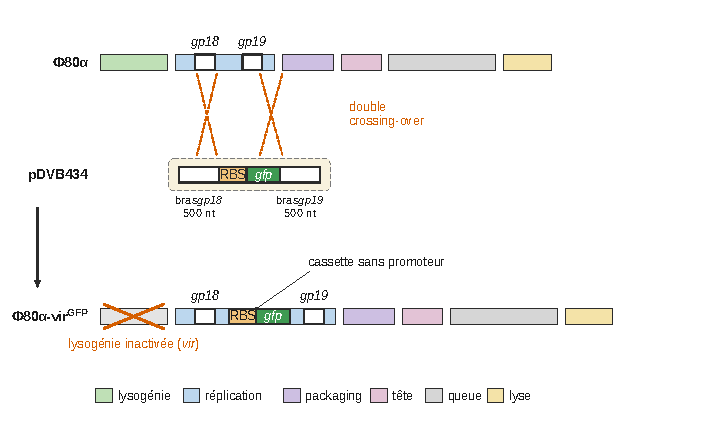
\includegraphics{figures/q5-genome-virgfp.pdf}
\caption*{Figure 1 --- Construction de Φ80α-virGFP : double crossing-over entre
les bras de 500 nt de pDVB434 et les séquences gp18 et gp19, insertion
de la cassette RBS-gfp dépourvue de promoteur, module de lysogénie
inactivé par la mutation vir}
\end{figure}

La cassette \textbf{RBS-\emph{gfp}} est insérée entre \emph{gp18} et \emph{gp19}, sans promoteur propre ; le module de lysogénie (\emph{cI}, \emph{int}) est rendu non fonctionnel par la mutation \emph{vir}, d'où un phage \textbf{exclusivement lytique}, comme l'annonce l'énoncé.

\equationajustee{\boxed{\text{pDVB434 = matrice de recombinaison : 2 bras de 500 nt (adressage) + RBS (traduction) + }\textit{gfp}\text{ (rapporteur), sans promoteur.}}}

\hypertarget{q6.-fonctionnement-de-crispr-cas9-et-uxe9limination-des-phages-non-recombinants}{%
\subsection{Q6. Fonctionnement de CRISPR-Cas9 et élimination des phages non recombinants}\label{q6.-fonctionnement-de-crispr-cas9-et-uxe9limination-des-phages-non-recombinants}}

\textbf{a. Fonctionnement du système.} Le système CRISPR-Cas de type II est, dans son contexte naturel, un \textbf{système immunitaire adaptatif bactérien} dirigé contre les acides nucléiques étrangers, phages compris. Il repose sur deux composants :

\begin{itemize}
\tightlist
\item
  une \textbf{endonucléase Cas9}, protéine bilobée à deux domaines catalytiques (RuvC et HNH), chacun coupant un brin ;
\item
  un \textbf{ARN guide}, chimère du crRNA --- dont une vingtaine de nucléotides sont complémentaires de la cible --- et du tracrRNA, qui assure le repliement et l'ancrage sur Cas9.
\end{itemize}

Le complexe Cas9--ARN guide balaie l'ADN à la recherche d'un motif court adjacent à la cible, le \textbf{PAM} (\emph{Protospacer Adjacent Motif}), dont la séquence est propre à chaque orthologue de Cas9 (5′-NGG-3′ pour celui de \emph{Streptococcus pyogenes}, 5′-NNGRRT-3′ pour celui de \textbf{\emph{S. aureus}}, qui est le système porté par pDVB435). En présence d'un PAM, l'ADN est localement déroulé, le guide s'apparie au brin complémentaire et, si l'appariement est correct, les deux domaines catalytiques coupent : il en résulte une \textbf{cassure double brin à bouts francs}, trois paires de bases en amont du PAM.

\textbf{b. Élimination des phages non recombinants.} À l'issue de l'étape 2, la descendance phagique est une population \textbf{mixte} : une minorité de recombinants ayant intégré la cassette RBS-\emph{gfp}, et une écrasante majorité de parentaux Φ80α-vir n'ayant pas recombiné, la recombinaison homologue étant un événement rare (de l'ordre de 10⁻⁴ à 10⁻⁶). Un criblage individuel par fluorescence serait hors de portée.

Le plasmide pDVB435 porte un système CRISPR-Cas9 ciblant « uniquement une séquence spécifique du bactériophage Φ80α », en l'occurrence la séquence du point d'insertion. Lorsque, à l'\textbf{étape 3}, ces phages infectent \emph{S. aureus}-pDVB435 :

\begin{itemize}
\tightlist
\item
  chez un \textbf{phage non recombinant}, la séquence cible est intacte : Cas9 la reconnaît, coupe le génome viral en double brin, et le cycle avorte. Le phage ne se multiplie pas et ne forme pas de plage ;
\item
  chez un \textbf{phage recombinant}, l'insertion de la cassette a détruit ou déplacé la séquence cible et son PAM : le guide ne trouve plus d'appariement, Cas9 ne coupe pas, le génome est répliqué et encapsidé normalement.
\end{itemize}

La coupure est \textbf{létale pour le phage} parce que, dans ce contexte, elle n'est pas réparée : \emph{S. aureus} ne possède pas de voie de jonction d'extrémités non homologues, et le génome viral coupé ne dispose d'aucune matrice homologue utilisable. (La recombinaison homologue bactérienne, elle, existe bel et bien : c'est elle qui a réalisé l'insertion à l'étape 2.)

Le système réalise donc une \textbf{contre-sélection} : il n'avantage pas les recombinants, il élimine tout le reste. Le tri s'opère à l'étape 3, de sorte que les phages \textbf{récupérés et concentrés à l'étape 4 sont pratiquement tous des Φ80α-virGFP}, sans criblage individuel.

\equationajustee{\boxed{\text{Cas9 coupe le \text{génome} des phages ayant \text{conservé} la cible ; seuls les recombinants, dont la cible est \text{remplacée} par RBS-}\textit{gfp}\text{, se multiplient.}}}

\hypertarget{q7.-obtenir-des-phages-lytiques-ux3c680ux3b1-vir-uxe0-partir-de-ux3c680ux3b1}{%
\subsection{Q7. Obtenir des phages lytiques Φ80α-vir à partir de Φ80α}\label{q7.-obtenir-des-phages-lytiques-ux3c680ux3b1-vir-uxe0-partir-de-ux3c680ux3b1}}

\textbf{Cible moléculaire.} Le caractère tempéré de Φ80α repose sur le module de lysogénie identifié en Q1 ; la bascule lyse/lysogénie est gouvernée par le \textbf{répresseur CI}, qui occupe les opérateurs et réprime les gènes lytiques précoces. Un mutant \emph{vir} est un mutant \textbf{insensible à la répression}. Rendre le phage strictement lytique revient donc à \textbf{supprimer la fonction CI} et, pour être complet, à supprimer également l'\textbf{intégrase} \emph{int}, ce qui interdit physiquement l'intégration au chromosome.

\textbf{Méthode proposée --- remplacement allélique par recombinaison homologue, puis contre-sélection CRISPR} (transposition de la stratégie du document 3) :

\begin{enumerate}
\def\labelenumi{\arabic{enumi}.}
\tightlist
\item
  \textbf{Construire un plasmide} portant deux bras d'homologie d'environ 500 nt correspondant aux régions flanquant \emph{cI}--\emph{int}, encadrant une délétion ou une courte séquence de substitution (codons stop dans les trois cadres).
\item
  \textbf{Transformer} \emph{S. aureus} RN4220 par ce plasmide.
\item
  \textbf{Infecter} cette souche par Φ80α sauvage : pendant le cycle lytique, une fraction rare des génomes viraux subit un double crossing-over et perd \emph{cI} (et \emph{int}).
\item
  \textbf{Récupérer la descendance} et en \textbf{infecter une seconde souche} transformée par un plasmide CRISPR-Cas9 dont le guide cible la séquence \emph{cI} sauvage : les phages ayant conservé \emph{cI} sont coupés et éliminés, seuls les phages délétés se multiplient.
\item
  \textbf{Vérifier} le phénotype par trois critères indépendants : plages de lyse \textbf{claires} et non troubles, absence de formation de lysogènes sur boîte, et incapacité à être bloqué par une souche lysogène pour Φ80α.
\end{enumerate}

\textbf{Variante par enzymes de restriction.} Le même objectif --- supprimer les séquences codant la lysogénie --- s'atteint par digestion du génome viral purifié au moyen d'enzymes de restriction encadrant le module \emph{cI}--\emph{int}, religature du génome délété, puis transfection de la souche hôte. La méthode est plus grossière (elle dépend de la présence de sites uniques bien placés) mais elle ne demande ni plasmide de recombinaison ni système CRISPR.

\textbf{Méthode alternative, sans génie génétique.} Historiquement, les mutants \emph{vir} s'obtiennent par \textbf{sélection de mutants spontanés} : on étale une forte quantité de phages sauvages sur un tapis d'une souche \textbf{lysogène} pour Φ80α, immunisée par le CI qu'elle produit. Seuls les rares mutants insensibles à CI (mutations des opérateurs) forment des plages, que l'on repique. Rendement faible et mutation non contrôlée, mais aucun outil moléculaire requis ; une mutagenèse préalable (UV, agent alkylant) augmente la fréquence au prix de mutations secondaires.

\equationajustee{\boxed{\text{Inactiver } \textit{cI} \text{ (et } \textit{int}\text{) par recombinaison homologue plasmidique, puis contre-\text{sélectionner} par CRISPR-Cas9 ciblant } \textit{cI}.}}

\hypertarget{staphylococcus-aureus-rn4220}{%
\subsection{\texorpdfstring{3. \emph{Staphylococcus aureus} RN4220}{3. Staphylococcus aureus RN4220}}\label{staphylococcus-aureus-rn4220}}

\hypertarget{q8.-analyse-fonctionnelle-du-milieu-bhi-broth}{%
\subsection{Q8. Analyse fonctionnelle du milieu BHI Broth}\label{q8.-analyse-fonctionnelle-du-milieu-bhi-broth}}

Le bouillon BHI (\emph{Brain Heart Infusion}) est un milieu \textbf{liquide, complexe (non synthétique), riche, tamponné et non sélectif}.

\begin{longtable}[]{@{}
  >{\raggedright\arraybackslash}p{(\columnwidth - 4\tabcolsep) * \real{0.2141}}
  >{\raggedright\arraybackslash}p{(\columnwidth - 4\tabcolsep) * \real{0.3339}}
  >{\raggedright\arraybackslash}p{(\columnwidth - 4\tabcolsep) * \real{0.4221}}@{}}
\toprule\noalign{}
\begin{minipage}[b]{\linewidth}\raggedright
Constituant (pour 1 L)
\end{minipage} & \begin{minipage}[b]{\linewidth}\raggedright
Nature / apport chimique
\end{minipage} & \begin{minipage}[b]{\linewidth}\raggedright
Rôle fonctionnel
\end{minipage} \\
\midrule\noalign{}
\endhead
\bottomrule\noalign{}
\endlastfoot
Peptone --- 10,0 g & Hydrolysat enzymatique de protéines : peptides courts, acides aminés libres & Source d'\textbf{azote} organique et de \textbf{carbone} directement assimilable ; fournit les acides aminés que \emph{S. aureus}, auxotrophe pour plusieurs d'entre eux, ne sait pas synthétiser \\
Infusion de cervelle de veau --- 12,5 g & Extrait tissulaire : peptides, acides aminés, lipides, vitamines du groupe B, bases azotées, oligo-éléments & Apport de \textbf{facteurs de croissance} non substituables ; permet la culture de bactéries exigeantes \\
Infusion de cœur de bœuf --- 5,0 g & Extrait tissulaire complémentaire (nucléotides, minéraux, hème) & Même rôle ; la combinaison des deux infusions élargit le spectre des facteurs apportés \\
Chlorure de sodium --- 5,0 g & Sels minéraux : Na⁺, Cl⁻ (≈ 86 mmol·L⁻¹) & Maintien de la \textbf{pression osmotique} et de l'\textbf{équilibre ionique} ; à 0,5 \%, cette concentration n'a aucun effet sélectif \\
Hydrogénophosphate disodique anhydre --- 2,5 g & Couple tampon HPO₄²⁻/H₂PO₄⁻ (p\(K_{a2} \approx 7{,}2\)), ≈ 18 mmol·L⁻¹ & \textbf{Double rôle} : pouvoir tampon limitant l'acidification due à la fermentation du glucose, et source de \textbf{phosphore} (acides nucléiques, ATP, phospholipides) \\
Glucose --- 2,0 g & Ose simple, ≈ 11 mmol·L⁻¹ & \textbf{Source de carbone et d'énergie} rapidement métabolisable (glycolyse) ; soutient la croissance exponentielle rapide exigée par le protocole (phase exponentielle en ≈ 90 min) \\
Eau distillée --- q.s.p. 1 000 mL & Solvant purifié, exempt d'ions parasites & \textbf{Solvant} de tous les constituants ; assure l'activité de l'eau et le transport des solutés \\
pH final 7,4 ± 0,2 à 25 °C & Paramètre physico-chimique & pH \textbf{neutre}, optimal pour \emph{S. aureus} (neutrophile) et compatible avec la stabilité des virions \\
\end{longtable}

\textbf{Conclusion.} Aucun constituant n'est inhibiteur ni indicateur : le BHI est un milieu \textbf{d'enrichissement non sélectif et non différentiel}, adapté à la production d'une forte biomasse en phase exponentielle, c'est-à-dire de cellules hôtes métaboliquement actives --- exactement ce qu'exige la production de phages. Le complément de \textbf{5 mM CaCl₂} du document 2 n'appartient pas à la formule de base et n'a pas de rôle nutritionnel : il sert à l'\textbf{adsorption phagique}.

\hypertarget{q9.-adaptation-du-milieu-pour-les-souches-ogm}{%
\subsection{Q9. Adaptation du milieu pour les souches OGM}\label{q9.-adaptation-du-milieu-pour-les-souches-ogm}}

Le document 4 indique que les deux souches modifiées, RN4220::\emph{Ssc}-CBASS-cmᴿ et RN4220::\emph{Ssc}-CdnE03-cmᴿ, portent toutes deux, intégrée au chromosome, une séquence \textbf{cmᴿ} codant la \textbf{résistance au chloramphénicol}. La souche sauvage en est dépourvue : le marqueur de sélection est donc fourni par l'énoncé.

\textbf{Adaptation proposée.} Ajouter au bouillon BHI du \textbf{chloramphénicol} à concentration sélective, soit environ \textbf{10 µg·mL⁻¹} pour \emph{S. aureus} (usuellement 5 à 15 µg·mL⁻¹). L'antibiotique étant \textbf{thermolabile}, il ne doit pas être autoclavé : on prépare une solution mère concentrée dans l'éthanol, on la \textbf{stérilise par filtration à 0,22 µm} et on l'ajoute au milieu \textbf{après} autoclavage et refroidissement en dessous de 50 °C.

\textbf{Justification du couple mécanisme / sélection.} Le chloramphénicol est un inhibiteur de la \textbf{traduction} : il se fixe sur le centre peptidyl-transférase de la sous-unité \textbf{50S} du ribosome bactérien et bloque la formation de la liaison peptidique ; il est \textbf{bactériostatique}, à large spectre. Le gène cmᴿ code une \textbf{chloramphénicol acétyltransférase}, qui acétyle l'antibiotique et l'empêche de se fixer au ribosome.

\begin{itemize}
\tightlist
\item
  \textbf{Souches OGM} : elles produisent l'acétyltransférase, inactivent l'antibiotique et \textbf{croissent normalement}.
\item
  \textbf{Souche sauvage} : dépourvue de cmᴿ, sa traduction est bloquée et sa \textbf{croissance est empêchée}, ce qu'exige l'énoncé.
\end{itemize}

\textbf{Deux réserves.} D'abord, le chloramphénicol étant \textbf{bactériostatique} et non bactéricide, il inhibe la souche sauvage sans la tuer : des cellules sauvages viables peuvent persister. Pour une élimination stricte, il faudrait augmenter la concentration, enchaîner des repiquages sélectifs ou choisir un marqueur bactéricide. Ensuite, ce milieu ne convient qu'à la \textbf{culture des souches} : le chloramphénicol bloquerait aussi la traduction des protéines virales et fausserait l'étude du CBASS. Il faut donc cultiver les OGM en BHI + chloramphénicol, puis \textbf{laver et transférer} les cellules en BHI sans antibiotique avant toute infection --- c'est bien ce que fait le document 10, où seul du BHI + CaCl₂ est ajouté.

\equationajustee{\boxed{\text{BHI Broth} + \text{\text{chloramphénicol}} \approx 10\ \mu\text{g}\cdot\text{mL}^{-1},\ \text{\text{filtré} \text{à} } 0{,}22\ \mu\text{m et \text{ajouté} \text{après} autoclavage.}}}

\hypertarget{q10.-allure-des-courbes-de-croissance-dans-les-trois-cas}{%
\subsection{Q10. Allure des courbes de croissance dans les trois cas}\label{q10.-allure-des-courbes-de-croissance-dans-les-trois-cas}}

Les trois cultures sont conduites en BHI Broth, à 37 °C, la densité optique à 600 nm étant portée en échelle logarithmique en fonction du temps. L'infection est réalisée à MOI = 0,1.

\begin{figure}[H]
\centering
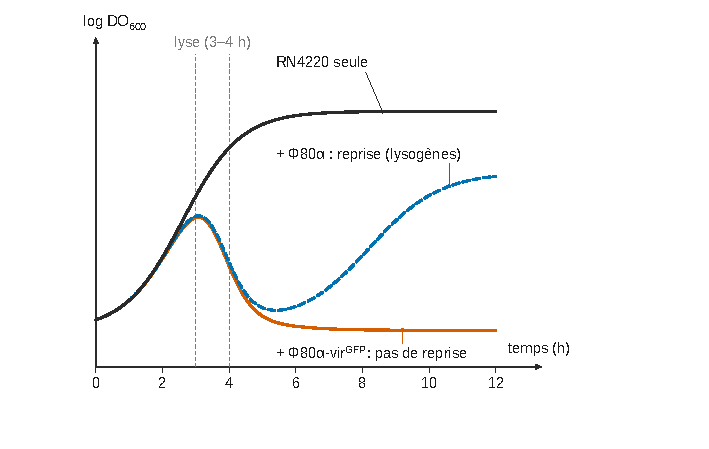
\includegraphics{figures/q10-courbes-croissance.pdf}
\caption*{Figure 2 --- Allure des trois courbes de croissance : chute de la DO₆₀₀
vers 3--4 h dans les deux cultures infectées, reprise seulement avec le
phage tempéré Φ80α}
\end{figure}

\textbf{Cas 1 --- RN4220 sauvage seule (témoin).} Courbe de croissance canonique en milieu non renouvelé : \textbf{phase de latence} courte (milieu riche, inoculum issu d'une préculture, adaptation enzymatique minimale), \textbf{phase exponentielle} de pente maximale (temps de génération de \emph{S. aureus} en BHI à 37 °C : ≈ 25--30 min), \textbf{ralentissement} puis \textbf{phase stationnaire} lorsque le glucose s'épuise et que les produits acides s'accumulent, enfin déclin lent.

\textbf{Cas 2 --- RN4220 + Φ80α (phage tempéré).} Jusqu'à ≈ 2 h, la courbe est superposable au témoin : à MOI = 0,1, une bactérie sur dix seulement est initialement infectée et la croissance des non infectées masque la lyse. Après deux à trois cycles infectieux successifs (cycle de ≈ 30--45 min), la lyse devient synchrone à l'échelle de la population et la \textbf{densité optique s'effondre} --- c'est la « perte totale de turbidité » observée à 3--4 h dans le document 2. \textbf{Mais la chute n'est pas définitive} : Φ80α étant \textbf{tempéré}, une fraction des cellules infectées est entrée en lysogénie. Ces lysogènes portent le prophage, expriment CI et bénéficient de l'\textbf{immunité de superinfection} : insensibles aux virions libres, ils repartent en croissance et la DO \textbf{remonte} après quelques heures. S'y ajoutent les mutants d'adsorption (récepteur pariétal altéré) sélectionnés par la pression phagique.

\textbf{Cas 3 --- RN4220 + Φ80α-virGFP (phage strictement lytique).} Le début et la chute sont identiques (même hôte, même MOI, même cycle lytique). \textbf{La différence est en aval} : ce phage étant exclusivement lytique (module de lysogénie inactivé, Q5 et Q7), \textbf{aucun lysogène ne peut se former}. Aucune sous-population immunisée ne subsiste et la \textbf{DO reste basse durablement}. Seule une repousse tardive de mutants d'adsorption pourrait apparaître, plus lente et plus rare.

\begin{longtable}[]{@{}
  >{\raggedright\arraybackslash}p{(\columnwidth - 6\tabcolsep) * \real{0.2597}}
  >{\raggedright\arraybackslash}p{(\columnwidth - 6\tabcolsep) * \real{0.1732}}
  >{\raggedright\arraybackslash}p{(\columnwidth - 6\tabcolsep) * \real{0.2499}}
  >{\raggedright\arraybackslash}p{(\columnwidth - 6\tabcolsep) * \real{0.2872}}@{}}
\toprule\noalign{}
\begin{minipage}[b]{\linewidth}\raggedright
\end{minipage} & \begin{minipage}[b]{\linewidth}\raggedright
RN4220 seule
\end{minipage} & \begin{minipage}[b]{\linewidth}\raggedright
+ Φ80α
\end{minipage} & \begin{minipage}[b]{\linewidth}\raggedright
+ Φ80α-virGFP
\end{minipage} \\
\midrule\noalign{}
\endhead
\bottomrule\noalign{}
\endlastfoot
Croissance initiale (0--2 h) & normale & normale & normale \\
Chute de DO & absente & marquée, vers 3--4 h & marquée, vers 3--4 h \\
Reprise ultérieure & --- & \textbf{oui} (lysogènes immunisés) & \textbf{non} (sauf mutants rares, tardifs) \\
DO finale & maximale & intermédiaire & minimale \\
\end{longtable}

\textbf{Précision indispensable.} La densité optique mesure une \textbf{turbidité}, donc la biomasse totale, cellules vivantes \emph{et} cellules mortes non lysées : elle ne se confond pas avec un dénombrement de bactéries viables.

\equationajustee{\boxed{\text{\text{Témoin} : croissance \text{complète}. Φ80α : lyse puis }\textbf{reprise}\text{ (\text{lysogènes}). Φ80α-virGFP : lyse }\textbf{sans reprise}\text{ (phage }\textit{vir}\text{).}}}

\hypertarget{q11.-intuxe9gration-chromosomique-plutuxf4t-que-plasmide-recombinant}{%
\subsection{Q11. Intégration chromosomique plutôt que plasmide recombinant}\label{q11.-intuxe9gration-chromosomique-plutuxf4t-que-plasmide-recombinant}}

Le document 4 porte la mention « \emph{chromosomal integration} » : les séquences \emph{Ssc}-CdnE03 ou \emph{Ssc}-CBASS ont été insérées dans le chromosome bactérien.

\textbf{Avantages de l'intégration chromosomique.}

\begin{itemize}
\tightlist
\item
  \textbf{Stabilité génétique.} Le chromosome est répliqué et ségrégé fidèlement à chaque division, alors qu'un plasmide se perd par ségrégation aléatoire en l'absence de pression de sélection. C'est l'argument \textbf{décisif ici} : les expériences du document 10 durent 12 h, sans antibiotique dans le milieu (qui fausserait l'infection) ; seule l'intégration chromosomique garantit que toutes les bactéries observées portent encore le système.
\item
  \textbf{Nombre de copies unique et défini.} Une copie par chromosome donne un niveau d'expression \textbf{physiologique}, comparable à celui du système natif. Un plasmide à 5, 20 ou 200 copies surexprimerait le système d'autant, au risque de créer artificiellement une immunité que la bactérie sauvage n'a pas : le phénotype observé ne serait plus qu'un artefact de dosage génique, inacceptable pour l'étude d'un mécanisme physiologique de défense.
\item
  \textbf{Pas de charge métabolique ni de dissémination.} Pas de réplication plasmidique à financer, donc pas de biais de croissance ; et pas de transfert horizontal possible du système ou du marqueur de résistance.
\end{itemize}

\textbf{Inconvénients.}

\begin{itemize}
\tightlist
\item
  \textbf{Construction lourde et lente} : vecteur suicide ou recombinaison site-spécifique, sélection des intégrants, vérification du site par PCR et séquençage --- là où une transformation plasmidique est affaire de quelques heures.
\item
  \textbf{Faible niveau d'expression} : la copie unique peut rendre difficile la détection biochimique de la protéine ou sa purification, que facilite un plasmide multicopie.
\item
  \textbf{Modification peu réversible et non transférable} : on ne « cure » pas une insertion chromosomique comme on perd un plasmide, et on ne la transfère pas telle quelle à une autre souche.
\item
  \textbf{Effet de position} : l'insertion peut interrompre un gène ou perturber l'expression des gènes voisins ; il faut vérifier que le phénotype vient bien de la construction et non de la lésion créée.
\end{itemize}

\equationajustee{\boxed{\text{\text{Stabilité} sans antibiotique + copie unique (expression physiologique) ; mais construction lourde, expression faible, effet de position.}}}

\hypertarget{q12-ruxe9dactionnelle.-diversituxe9-structurale-des-virus-cycle-viral-mise-en-uxe9vidence-et-quantification}{%
\subsection{Q12 (rédactionnelle). Diversité structurale des virus, cycle viral, mise en évidence et quantification}\label{q12-ruxe9dactionnelle.-diversituxe9-structurale-des-virus-cycle-viral-mise-en-uxe9vidence-et-quantification}}

\textbf{Introduction.} Un virus est une \textbf{entité biologique acellulaire}, \textbf{parasite intracellulaire obligatoire}, dépourvue de métabolisme propre et de machinerie de traduction. Il se réduit à un génome --- un seul type d'acide nucléique, ADN \textbf{ou} ARN --- protégé par une coque protéique, la capside, l'ensemble formant la \textbf{nucléocapside}, parfois entourée d'une enveloppe lipidique empruntée aux membranes de l'hôte. Le bactériophage Φ80α étudié ici en est un représentant, mais il n'illustre qu'une des morphologies possibles. Nous montrerons d'abord l'ampleur de la diversité structurale des virus, puis que cette diversité recouvre un schéma fonctionnel commun, le cycle viral, et nous proposerons enfin une méthode permettant de détecter et de quantifier spécifiquement un virus au cours d'une infection.

\textbf{I. Une diversité structurale considérable, organisée par quatre critères}

\emph{1. Nature et topologie du génome.} C'est le critère fondateur de la classification de Baltimore. Le génome peut être de l'\textbf{ADN double brin} (Φ80α, Adénovirus, virus de l'herpès), de l'\textbf{ADN simple brin} (Parvovirus B19, phage M13), de l'\textbf{ARN double brin} (Rotavirus), de l'\textbf{ARN simple brin de polarité positive}, directement traduisible comme un ARN messager (Poliovirus, SARS-CoV-2), ou de l'\textbf{ARN simple brin de polarité négative}, qui impose au virus d'emporter sa propre ARN polymérase ARN-dépendante dans le virion (virus de la grippe, de la rage, Ebola). Les \textbf{rétrovirus} (VIH) ont un ARN positif rétrotranscrit en ADN par une transcriptase inverse. La topologie varie aussi : génome \textbf{linéaire} (Φ80α, Adénovirus) ou \textbf{circulaire} (phage φX174) ; \textbf{monopartite} ou \textbf{segmenté} --- les huit segments du virus de la grippe A autorisent des réassortiments entre souches, à l'origine des pandémies.

\emph{2. Symétrie de la capside.}

\begin{itemize}
\tightlist
\item
  \textbf{Symétrie icosaédrique} : polyèdre régulier à 20 faces triangulaires, construit par autoassemblage de capsomères identiques --- l'architecture la plus économe en information génétique (Adénovirus, Poliovirus, Papillomavirus).
\item
  \textbf{Symétrie hélicoïdale} : les protomères s'enroulent autour du génome en une hélice dont la longueur est fixée par celle de l'acide nucléique. Exemple canonique : le virus de la mosaïque du tabac, bâtonnet rigide de 300 nm ; les virus de la grippe et de la rage ont une nucléocapside hélicoïdale souple, repliée dans une enveloppe.
\item
  \textbf{Symétrie complexe ou mixte} : les \textbf{phages caudés} comme Φ80α associent une tête icosaédrique et une queue hélicoïdale à fibres ; les Poxvirus (variole) sont des briques de 300 nm sans symétrie régulière.
\end{itemize}

\emph{3. Présence ou absence d'enveloppe.} Les virus \textbf{nus} (Φ80α, Poliovirus, Adénovirus, Norovirus) n'ont pas de bicouche lipidique : ils résistent à la dessiccation, aux solvants organiques et aux détergents, d'où leur transmission féco-orale et leur persistance dans l'environnement --- et, dans ce sujet, la possibilité de conserver le lysat à 4 °C après filtration. Les virus \textbf{enveloppés} (VIH, grippe, SARS-CoV-2, herpès) portent une membrane dérivée de l'hôte, hérissée de glycoprotéines : fragiles hors de l'organisme, mais capables d'entrer par fusion membranaire et partiellement camouflés vis-à-vis de l'immunité.

\emph{4. Taille.} De ≈ 20 nm (Parvovirus) à ≈ 300 nm (Poxvirus) et jusqu'à ≈ 700 nm pour le Mimivirus, plus gros qu'une petite bactérie ; 30 nm pour un Poliovirus, 100 nm pour le VIH, 60--200 nm pour un phage caudé. Presque tous restent en deçà du pouvoir de résolution du microscope optique, d'où le recours à la microscopie électronique pour les observer.

\begin{lstlisting}
Quatre morphotypes
  (a) icosaédrique nu : capside polyédrique, pas d'enveloppe        (Adénovirus)
  (b) hélicoïdal nu   : bâtonnet rigide, protomères en hélice        (TMV)
  (c) enveloppé       : nucléocapside + bicouche + spicules          (SARS-CoV-2)
  (d) complexe caudé  : tête icosaédrique + queue + fibres           (Φ80α)
\end{lstlisting}

\textbf{II. Une unité fonctionnelle : les grandes étapes du cycle viral}

Quelle que soit sa structure, tout virus, incapable de produire son ATP et de traduire ses ARN, doit détourner une cellule. Le cycle se décompose universellement en six étapes.

\begin{enumerate}
\def\labelenumi{\arabic{enumi}.}
\tightlist
\item
  \textbf{Attachement (adsorption).} Une protéine de surface du virion --- fibres caudales chez Φ80α, protéine Spike chez le SARS-CoV-2, gp120 chez le VIH --- reconnaît spécifiquement un \textbf{récepteur} de la cellule cible : acide teichoïque de la paroi staphylococcique, enzyme de conversion de l'angiotensine 2, molécule CD4. Cette reconnaissance détermine le \textbf{tropisme}. Chez les phages, l'adsorption exige souvent des cations divalents, d'où les 5 mM de CaCl₂ du document 2.
\item
  \textbf{Pénétration et décapsidation.} Un phage caudé \textbf{injecte} son seul ADN à travers la paroi et la membrane, la capside vide restant à l'extérieur ; un virus nu animal entre par \textbf{endocytose} ; un virus enveloppé entre par \textbf{fusion} de son enveloppe avec la membrane plasmique ou endosomale. Dans les deux derniers cas, une \textbf{décapsidation} libère ensuite le génome.
\item
  \textbf{Expression précoce et détournement de la cellule.} Sont produites les protéines non structurales : polymérases, protéines de réplication, protéines d'inhibition des défenses de l'hôte. Chez Φ80α, c'est le moment de la bascule CI/Cro qui décide de la lyse ou de la lysogénie, et c'est aussi celui où s'exprime la cassette \emph{gfp} du phage rapporteur.
\item
  \textbf{Réplication du génome}, selon une stratégie propre à chaque classe de Baltimore : réplication semi-conservative pour les virus à ADN, ARN polymérase ARN-dépendante virale pour les virus à ARN, transcription inverse puis intégration pour les rétrovirus. Elle est massivement amplificatrice.
\item
  \textbf{Assemblage et maturation.} L'\textbf{expression tardive} fournit les protéines de structure ; les capsides s'autoassemblent, puis le génome est encapsidé --- chez Φ80α, par translocation active à travers le portail sous l'action de la terminase TerS/TerL, avant fixation de la queue préassemblée. Des \textbf{clivages protéolytiques} de maturation rendent le virion infectieux.
\item
  \textbf{Libération.} Soit la \textbf{lyse}, brutale et létale --- chez Φ80α, l'holine perméabilise la membrane et l'endolysine hydrolyse le peptidoglycane, libérant d'un coup une centaine de virions ; soit le \textbf{bourgeonnement}, progressif, qui laisse la cellule survivre un temps (VIH, grippe). Une voie particulière est le \textbf{cycle lysogénique} des phages tempérés, où le génome s'intègre au chromosome et se transmet verticalement jusqu'à une induction ultérieure.
\end{enumerate}

\textbf{III. Détecter et quantifier spécifiquement un virus : la RT-qPCR}

Deux logiques coexistent. La \textbf{quantification du pouvoir infectieux} repose sur des méthodes biologiques : \textbf{dénombrement sur gélose avec plages de lyse} pour un phage (PFU·mL⁻¹, questions Q3--Q4), dose infectieuse 50 \% en culture cellulaire pour un virus animal ; spécifiques d'une activité, mais lentes et inapplicables à un virus non cultivable. La \textbf{quantification des particules ou des génomes} repose sur des méthodes moléculaires ou immunologiques, plus rapides et plus sensibles : \textbf{qPCR} ou \textbf{RT-qPCR}, \textbf{hybridation par sonde moléculaire}, \textbf{ELISA} dirigé contre une protéine de capside, \textbf{microscopie} électronique ou à immunofluorescence pour un comptage direct de particules. C'est la seconde famille que nous détaillons, en retenant la méthode la plus spécifique et la plus quantitative.

\emph{Principe.} La \textbf{RT-qPCR} (transcription inverse suivie d'une PCR quantitative en temps réel) détecte et dénombre les génomes viraux. Sa \textbf{spécificité} repose sur trois reconnaissances moléculaires : le couple d'\textbf{amorces}, choisi dans une région du génome propre au virus recherché et absente de l'hôte ; la \textbf{sonde d'hydrolyse} interne, marquée par un fluorochrome émetteur et un extincteur ; et la \textbf{température d'hybridation}, ajustée au \(T_m\) des amorces.

\emph{Déroulement.} Extraction des acides nucléiques de l'échantillon ; \textbf{transcription inverse} de l'ARN viral en ADN complémentaire (étape omise pour un virus à ADN, on parle alors de qPCR) ; \textbf{amplification} sur une quarantaine de cycles de dénaturation (95 °C), hybridation (≈ 60 °C) et élongation. À chaque élongation, l'activité exonucléasique 5′→3′ de la polymérase hydrolyse la sonde : l'émetteur, séparé de l'extincteur, \textbf{émet}. La fluorescence croît donc avec le nombre d'amplicons.

\emph{Quantification.} On définit le \textbf{\(C_t\)}, numéro du cycle auquel la fluorescence franchit un seuil fixé au-dessus du bruit de fond. En régime exponentiel, \(Q_n = Q_0 (1+E)^n\) avec \(E\) l'efficacité, d'où une relation \textbf{affine} entre \(C_t\) et \(\log_{10} Q_0\) :

\equationajustee{C_t = -\frac{1}{\log_{10}(1+E)}\ \log_{10}(Q_0) + \text{constante}.}

La quantification est \textbf{absolue} si l'on établit une gamme d'étalonnage à partir de dilutions décimales d'un standard de concentration connue : la droite \(C_t = f(\log_{10} Q_0)\) a une pente de \(-3{,}32\) pour une efficacité de 100 \% (car \(\log_2 10 \approx 3{,}32\) cycles par décade), et l'on y reporte le \(C_t\) de l'échantillon. Elle est \textbf{relative} si l'on compare l'échantillon à un calibrateur.

\emph{Témoins obligatoires.} Témoin négatif d'extraction et témoin sans matrice (contamination), témoin positif, et \textbf{contrôle interne d'amplification} validant l'absence d'inhibiteurs de PCR.

\emph{Limites et méthodes complémentaires.} La RT-qPCR quantifie des \textbf{génomes}, non des \textbf{virions infectieux} : elle reste positive alors qu'il ne subsiste que des débris génomiques. Pour conclure à une infection productive, on l'associe à une méthode fonctionnelle (culture, plages de lyse) ou à la détection de protéines virales par \textbf{ELISA}. La \textbf{sérologie}, elle, témoigne d'un contact avec le virus mais ne quantifie pas le virus lui-même.

\textbf{Conclusion.} La diversité structurale des virus --- nature du génome, symétrie, enveloppe, taille --- masque une remarquable unité de fonction : tous suivent la même séquence attachement -- pénétration -- expression -- réplication -- assemblage -- libération, et tous imposent à l'hôte de fournir énergie et ribosomes. C'est cette unité qui rend les méthodes de détection transposables d'un virus à l'autre, et c'est elle aussi qui explique que les hôtes aient développé des défenses ciblant des étapes communes du cycle --- le système CBASS étudié ici en est un exemple, qui interrompt le cycle entre la réplication et la libération.

\begin{center}\rule{0.5\linewidth}{0.5pt}\end{center}

\hypertarget{partie-2.-uxe9tude-du-systuxe8me-immunitaire-cbass}{%
\section{Partie 2. Étude du système immunitaire CBASS}\label{partie-2.-uxe9tude-du-systuxe8me-immunitaire-cbass}}

\hypertarget{uxe9tude-de-la-structure-de-la-cyclase-ssc-cdne03}{%
\subsection{1. Étude de la structure de la cyclase Ssc-CdnE03}\label{uxe9tude-de-la-structure-de-la-cyclase-ssc-cdne03}}

\hypertarget{q13.-nature-et-caractuxe9ristiques-ioniques-de-k9-k13-et-r83}{%
\subsection{Q13. Nature et caractéristiques ioniques de K9, K13 et R83}\label{q13.-nature-et-caractuxe9ristiques-ioniques-de-k9-k13-et-r83}}

Dans la nomenclature employée, la lettre est le code à une lettre de l'acide aminé et le nombre sa position dans la chaîne polypeptidique.

\begin{itemize}
\tightlist
\item
  \textbf{K9 et K13 : deux lysines} (Lys). Chaîne latérale \(-(\mathrm{CH_2})_4-\mathrm{NH_3^+}\) : quatre carbones aliphatiques terminés par une \textbf{amine primaire} en position ε.
\item
  \textbf{R83 : une arginine} (Arg). Chaîne latérale \(-(\mathrm{CH_2})_3-\mathrm{NH}-\mathrm{C}(\mathrm{NH_2})_2^+\) : trois carbones terminés par un groupement \textbf{guanidinium}.
\end{itemize}

Ces trois résidus appartiennent à la famille des acides aminés \textbf{basiques}, à chaîne latérale chargée positivement.

\begin{longtable}[]{@{}
  >{\raggedright\arraybackslash}p{(\columnwidth - 8\tabcolsep) * \real{0.2015}}
  >{\raggedright\arraybackslash}p{(\columnwidth - 8\tabcolsep) * \real{0.1884}}
  >{\raggedright\arraybackslash}p{(\columnwidth - 8\tabcolsep) * \real{0.2617}}
  >{\raggedright\arraybackslash}p{(\columnwidth - 8\tabcolsep) * \real{0.1234}}
  >{\raggedright\arraybackslash}p{(\columnwidth - 8\tabcolsep) * \real{0.1951}}@{}}
\toprule\noalign{}
\begin{minipage}[b]{\linewidth}\raggedright
Résidu
\end{minipage} & \begin{minipage}[b]{\linewidth}\raggedright
Code 3 lettres
\end{minipage} & \begin{minipage}[b]{\linewidth}\raggedright
Groupement ionisable
\end{minipage} & \begin{minipage}[b]{\linewidth}\raggedright
p\(K_R\)
\end{minipage} & \begin{minipage}[b]{\linewidth}\raggedright
Charge à pH 7,4
\end{minipage} \\
\midrule\noalign{}
\endhead
\bottomrule\noalign{}
\endlastfoot
Lysine (K9, K13) & Lys & ε-ammonium \(-\mathrm{NH_3^+}\) & ≈ 10,5 & \(+1\) \\
Arginine (R83) & Arg & guanidinium & ≈ 12,5 & \(+1\) \\
\end{longtable}

\textbf{Justification quantitative.} La relation de Henderson-Hasselbalch, \(\mathrm{pH} = \mathrm{p}K_a + \log_{10}\big([\mathrm{A^-}]/[\mathrm{AH}]\big)\), donne pour la lysine à pH 7,4 :

\equationajustee{\begin{aligned}
\log_{10}\frac{[\mathrm{NH_2}]}{[\mathrm{NH_3^+}]} &= 7{,}4 - 10{,}5 \\
&= -3{,}1 \\
\frac{[\mathrm{NH_3^+}]}{[\mathrm{NH_2}]} &\approx 1{,}3\times10^{3}
\end{aligned}}

soit \textbf{plus de 99,9 \% de forme protonée}. Pour l'arginine, l'écart de 5,1 unités porte ce rapport à ≈ 10⁵ : la protonation est totale. Le guanidinium est en outre exceptionnellement stable, sa charge positive étant \textbf{délocalisée par résonance} sur ses trois azotes --- d'où son p\(K_a\) très élevé et sa charge permanente dans toutes les conditions physiologiques.

\equationajustee{\boxed{\text{K9 et K13 = lysines (ε-NH}_3^+\text{, p}K_R \approx 10{,}5\text{) ; R83 = arginine (guanidinium, p}K_R \approx 12{,}5\text{) ; charge } +1 \text{ chacun \text{à} pH 7,4.}}}

\hypertarget{q14.-argumentation-de-la-liaison-arn-cyclase}{%
\subsection{Q14. Argumentation de la liaison ARN -- cyclase}\label{q14.-argumentation-de-la-liaison-arn-cyclase}}

\textbf{Propriétés physico-chimiques de l'ARN.} Un ARN est un polymère de ribonucléotides unis par des \textbf{liaisons phosphodiester} 3′--5′. Chaque phosphate intercalé entre deux riboses porte une fonction acide de p\(K_{a} \approx 1\) : à pH physiologique, il est \textbf{totalement déprotoné} et porte une \textbf{charge négative}. Un ARN de \(n\) nucléotides porte donc environ \(n\) charges négatives régulièrement réparties : c'est un \textbf{polyanion linéaire de forte densité de charge}, et cette charge est \textbf{indépendante de la séquence}. Les bases azotées, aromatiques et globalement non chargées à ce pH, offrent en revanche des donneurs et accepteurs de liaison hydrogène et peuvent s'empiler. Le ribose porte un hydroxyle 2′, absent de l'ADN, qui impose la conformation A aux hélices et constitue un point de reconnaissance propre à l'ARN.

\textbf{Propriétés de la zone d'interaction (document 5).} La cartographie du potentiel électrostatique de surface montre une protéine globalement \textbf{acide} --- les zones rouges, de potentiel négatif, dominent --- à l'exception d'une \textbf{poche nettement bleue}, donc de potentiel \textbf{positif}, encadrée et désignée comme « zone d'interaction ARN-cyclase ». L'agrandissement attribue ce potentiel positif à la convergence spatiale des chaînes latérales de \textbf{K9, K13 et R83}, trois résidus éloignés dans la séquence primaire mais rapprochés par le repliement : le site est \textbf{discontinu}, créé par la structure tertiaire.

\textbf{Argumentation de la liaison.} Elle repose sur une \textbf{complémentarité électrostatique}.

\begin{itemize}
\tightlist
\item
  \textbf{Liaisons ioniques (ponts salins)} entre les ammoniums des lysines, le guanidinium de l'arginine et les oxygènes phosphate du squelette de l'ARN. Individuellement de l'ordre de quelques dizaines de kJ·mol⁻¹, leur multiplicité assure une forte affinité globale.
\item
  \textbf{Liaisons hydrogène} : le guanidinium est un donneur \textbf{bidentate}, capable de former deux liaisons hydrogène simultanées avec les deux oxygènes non pontants d'un même phosphate --- géométrie idéale, qui explique la fréquence des arginines dans les sites de liaison aux acides nucléiques.
\item
  \textbf{Contribution entropique} : la formation de chaque pont salin libère des molécules d'eau et des contre-ions auparavant ordonnés autour des deux partenaires.
\end{itemize}

\textbf{Deux corollaires.} D'une part, ces interactions portent sur le \textbf{squelette} et sont donc \emph{a priori} \textbf{non spécifiques de séquence} : la sélectivité observée plus loin (Q18) ne peut venir du seul contact électrostatique, mais de la \textbf{structure secondaire et tertiaire} de l'ARN ligand, qui doit s'ajuster géométriquement à la poche. D'autre part, la liaison est \textbf{sensible à la force ionique} : une forte concentration en sel écrante les charges et dissocie le complexe --- propriété que l'on exploitera pour \textbf{éluer} l'ARN de la colonne d'affinité (Q15).

\equationajustee{\boxed{\text{ARN polyanionique (phosphates \text{déprotonés})} \longleftrightarrow \text{poche basique (K9, K13, R83) : ponts salins et liaisons \text{hydrogène}, non \text{spécifiques} de \text{séquence}.}}}

\hypertarget{uxe9tude-de-laffinituxe9-de-la-cyclase-ssc-cdne03}{%
\subsection{2. Étude de l'affinité de la cyclase Ssc-CdnE03}\label{uxe9tude-de-laffinituxe9-de-la-cyclase-ssc-cdne03}}

\hypertarget{q15.-uxe9tapes-de-la-chromatographie-daffinituxe9-schuxe9ma-luxe9genduxe9-et-explicituxe9}{%
\subsection{Q15. Étapes de la chromatographie d'affinité (schéma légendé et explicité)}\label{q15.-uxe9tapes-de-la-chromatographie-daffinituxe9-schuxe9ma-luxe9genduxe9-et-explicituxe9}}

La chromatographie d'affinité est une méthode séparative fondée sur une \textbf{interaction biospécifique et réversible} entre un \textbf{ligand} greffé sur la phase stationnaire et l'espèce à purifier. Ici, l'objet purifié n'est pas la protéine mais son \textbf{partenaire} : le ligand immobilisé est la \textbf{cyclase Ssc-CdnE03}, et l'on recherche les \textbf{ARN} capables de s'y fixer.

\begin{figure}[H]
\centering
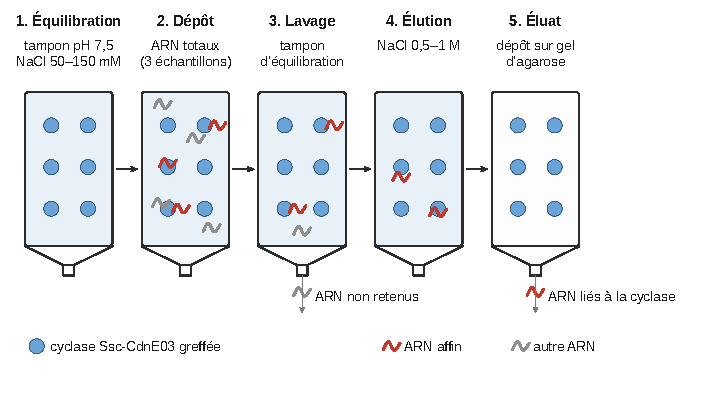
\includegraphics{figures/q15-chromatographie-affinite.pdf}
\caption*{Figure 3 --- Les cinq étapes de la chromatographie d'affinité : la
cyclase Ssc-CdnE03 est le ligand greffé, et l'élution par augmentation
de la force ionique fournit les ARN qui lui sont liés}
\end{figure}

\textbf{1. Préparation et équilibration.} La cyclase, produite par voie recombinante (le plus souvent avec une étiquette polyhistidine), est immobilisée sur la matrice --- couplage covalent sur résine activée, ou chélation par Ni²⁺-NTA. La colonne est rincée par le \textbf{tampon d'équilibration}, dont le pH et la force ionique rendent l'interaction possible : pH ≈ 7,5, où lysines et arginine sont protonées (Q13), et force ionique \textbf{faible} (50 à 150 mM NaCl), un excès de sel écrantant les charges et empêchant la fixation.

\textbf{2. Dépôt de l'échantillon.} On charge l'extrait d'\textbf{ARN totaux} de la condition testée (« -- », « RN4220 » ou « Φ80α »), à débit lent pour laisser l'équilibre de liaison s'établir. Les ARN reconnus par la poche basique s'y fixent, les autres traversent.

\textbf{3. Lavage.} Plusieurs volumes de colonne de tampon d'équilibration \textbf{éliminent les ARN non retenus et les interactions faibles ou non spécifiques}. Cette étape conditionne la pureté du résultat : un lavage insuffisant laisse un bruit de fond sur le gel, un lavage trop agressif décroche le ligand recherché.

\textbf{4. Élution.} On rompt volontairement l'interaction. Trois voies : \textbf{augmentation de la force ionique} (NaCl 0,5 à 1 M), qui écrante les interactions électrostatiques --- la voie la plus logique ici, compte tenu de la nature ionique de la liaison établie en Q14 ; \textbf{élution compétitive} par un excès de ligand libre ; ou \textbf{élution du complexe entier} par l'imidazole si le système repose sur une étiquette histidine, la protéine sortant alors avec son ARN. \textbf{C'est cette étape, et elle seule, qui fournit les ARN liés à la cyclase} demandés par l'énoncé.

\textbf{5. Récupération et analyse.} Les fractions d'élution sont collectées, éventuellement déprotéinisées et concentrées, puis déposées sur gel d'agarose : c'est le contenu du document 7.

\equationajustee{\boxed{\text{\text{équilibration}} \rightarrow \text{\text{dépôt}} \rightarrow \text{lavage} \rightarrow \textbf{\text{élution} (force ionique)} \rightarrow \text{\text{éluat} = ARN \text{liés} \text{à} la cyclase}}}

\hypertarget{q16.-polarituxe9-et-nom-des-uxe9lectrodes-e1-et-e2}{%
\subsection{Q16. Polarité et nom des électrodes E1 et E2}\label{q16.-polarituxe9-et-nom-des-uxe9lectrodes-e1-et-e2}}

\textbf{Charge de l'échantillon.} Comme établi en Q14, un ARN est un \textbf{polyanion} : dans le tampon d'électrophorèse (pH ≈ 8), tous ses phosphates sont déprotonés. La charge est proportionnelle à la longueur, donc le rapport charge/masse est \textbf{constant} : la migration ne dépend que de l'effet tamis de l'agarose, et \textbf{les molécules courtes migrent plus loin} que les longues.

\textbf{Sens de migration.} Un ion migre vers l'électrode de signe opposé au sien : les ARN, négatifs, migrent vers l'\textbf{anode}, pôle \textbf{positif} (en électrophorèse, régime imposé, l'anode est le pôle +, siège de l'oxydation).

\textbf{Lecture du document 7.} L'échelle de tailles décroît du haut vers le bas (2 000, 1 000, 500, 400, 200, 100, 50 nt) : les molécules les plus courtes sont donc les plus basses, la migration s'est faite \textbf{du haut vers le bas}, les puits de dépôt sont en haut, du côté de E1, et le front de migration en bas, du côté de E2.

\begin{longtable}[]{@{}llll@{}}
\toprule\noalign{}
Électrode & Position & Polarité & Nom \\
\midrule\noalign{}
\endhead
\bottomrule\noalign{}
\endlastfoot
E1 & haut, côté des puits & \(\ominus\) (négatif) & \textbf{cathode} \\
E2 & bas, côté du front & \(\oplus\) (positif) & \textbf{anode} \\
\end{longtable}

\equationajustee{\boxed{\text{E1 = cathode, \text{pôle} \text{négatif} ; E2 = anode, \text{pôle} positif.}}}

\hypertarget{q17.-intuxe9ruxeat-de-luxe9chantillon-darn-de-cellules-non-infectuxe9es-rn4220}{%
\subsection{Q17. Intérêt de l'échantillon d'ARN de cellules non infectées « RN4220 »}\label{q17.-intuxe9ruxeat-de-luxe9chantillon-darn-de-cellules-non-infectuxe9es-rn4220}}

L'échantillon « RN4220 » contient l'ARN total de bactéries \textbf{non infectées} : ARN ribosomiques (80 à 85 \% de l'ARN total), ARN de transfert, ARN messagers, petits ARN régulateurs. C'est un \textbf{témoin négatif biologique}, à distinguer du témoin « -- », qui est un témoin \emph{technique} sans aucun ARN.

Il permet de tester une hypothèse alternative précise : \textbf{la cyclase retient-elle n'importe quel ARN ?} La question est légitime, puisque l'interaction établie en Q14 est électrostatique et porte sur le squelette phosphate, commun à tous les ARN. Si la fixation n'était due qu'à la charge, les ARN bactériens abondants --- ARN ribosomiques 16S (≈ 1 540 nt) et 23S (≈ 2 900 nt) en tête --- seraient retenus et apparaîtraient sur le gel. Le témoin tranche donc entre deux interprétations :

\begin{itemize}
\tightlist
\item
  \textbf{si une bande apparaissait} dans cette piste, la fixation serait \textbf{non spécifique}, la colonne se comporterait comme un simple échangeur d'ions et la bande de la piste « Φ80α » n'aurait aucune signification biologique ;
\item
  \textbf{si aucune bande n'apparaît}, la cyclase ne retient pas les ARN de l'hôte non infecté, et toute bande observée en piste « Φ80α » est nécessairement liée à l'\textbf{infection}.
\end{itemize}

Ce témoin remplit donc trois fonctions : il contrôle la \textbf{spécificité} du ligand, il valide la \textbf{qualité du lavage}, et il fournit la \textbf{ligne de base biologique} de la comparaison. Il documente accessoirement l'absence d'\textbf{auto-immunité} du système : une cyclase qui se fixerait aux ARN de sa propre bactérie déclencherait en permanence la mort de celle-ci.

\equationajustee{\boxed{\text{\text{Témoin} \text{négatif} biologique : il \text{vérifie} que la cyclase ne fixe pas les ARN de l'\text{hôte}, donc que toute fixation \text{observée} est \text{spécifique} de l'infection.}}}

\hypertarget{q18.-analyse-du-gel-et-conclusion-sur-lactivation-de-la-cyclase}{%
\subsection{Q18. Analyse du gel et conclusion sur l'activation de la cyclase}\label{q18.-analyse-du-gel-et-conclusion-sur-lactivation-de-la-cyclase}}

\textbf{Analyse, piste par piste.}

\begin{itemize}
\tightlist
\item
  \textbf{Piste « -- » (sans ARN)} : aucune bande. La colonne ne libère par elle-même aucun acide nucléique : ni contamination, ni ARN coélué avec la protéine recombinante. Le contrôle technique est validé.
\item
  \textbf{Piste « RN4220 » (cellules non infectées)} : aucune bande visible. Bien que l'échantillon chargé contînt la totalité des ARN d'une bactérie, donc une immense majorité d'ARN ribosomiques, \textbf{aucun} n'a été retenu assez stablement pour se retrouver dans l'éluat.
\item
  \textbf{Piste « Φ80α » (cellules infectées)} : une bande \textbf{unique, fine et bien définie}, située entre les repères 500 et 1 000 nt et plus proche de 1 000, soit une taille d'environ \textbf{700 nt} (l'échelle étant logarithmique et la lecture graphique, on retiendra l'ordre de grandeur 600--800 nt). Le caractère unique et net de la bande est aussi informatif que sa présence : il exclut un mélange hétérogène et désigne \textbf{une seule espèce d'ARN}.
\end{itemize}

\textbf{Interprétation.} Les pistes 2 et 3 ne diffèrent que par un paramètre, la présence ou l'absence d'infection : l'ARN retenu est donc \textbf{apparu avec l'infection}. Deux origines restent possibles --- un \textbf{transcrit viral}, hypothèse la plus directe et celle des auteurs de l'étude, ou un ARN bactérien dont la transcription serait induite par l'infection. Le gel seul ne permet pas de trancher : il faudrait séquencer la bande. La conclusion mécanistique est la même dans les deux cas.

\textbf{Conclusion sur l'activation.} La cyclase Ssc-CdnE03 est une enzyme \textbf{dont l'activateur est un ARN spécifique produit lors de l'infection}. Elle fonctionne donc comme un \textbf{senseur moléculaire de l'infection} : en l'absence de phage, l'ARN activateur n'existe pas, la poche basique reste vide, l'enzyme est inactive et aucun nucléotide cyclique n'est produit ; dès l'infection, cet ARN s'accumule, se fixe dans la poche K9/K13/R83 et provoque le changement conformationnel \textbf{allostérique} qui organise le site catalytique. C'est le \textbf{premier maillon} de la cascade CBASS, celui de la \textbf{détection du non-soi}.

La sélectivité impose enfin une précision : le contact électrostatique de Q14 n'étant pas spécifique de séquence, elle provient nécessairement de la \textbf{structure secondaire et tertiaire} de cet ARN, que seul l'ARN viral adopte. La charge fournit l'énergie de liaison, la forme fournit la sélectivité.

\equationajustee{\boxed{\text{Un seul ARN, d'environ 700 nt, \text{présent} uniquement lors de l'infection, se fixe \text{à} la cyclase : la cyclase est un senseur \text{activé} par un ARN viral \text{spécifique}.}}}

\hypertarget{suivi-de-linfection-virale-et-de-la-ruxe9ponse-bactuxe9rienne-par-microscopie-uxe0-fluorescence}{%
\subsection{3. Suivi de l'infection virale et de la réponse bactérienne par microscopie à fluorescence}\label{suivi-de-linfection-virale-et-de-la-ruxe9ponse-bactuxe9rienne-par-microscopie-uxe0-fluorescence}}

\hypertarget{q19.-structures-secondaires-de-la-gfp-document-8a}{%
\subsection{Q19. Structures secondaires de la GFP (document 8a)}\label{q19.-structures-secondaires-de-la-gfp-document-8a}}

Le modèle tridimensionnel en rubans, présenté sous deux angles, code chaque type de structure par une forme et une couleur. On en identifie \textbf{trois}, qu'il faut nommer avec leur couleur.

\begin{itemize}
\tightlist
\item
  \textbf{Des feuillets β (en jaune)}, figurés par de larges flèches plates : \textbf{très majoritaires}, ils constituent l'ossature de la protéine. Les flèches voisines pointent en sens opposés : les brins sont \textbf{antiparallèles}, et ils sont \textbf{enroulés en cylindre fermé} --- les \textbf{11 brins β} du \textbf{tonneau β} de la GFP. Un feuillet β est stabilisé par des liaisons hydrogène \emph{inter-brins} entre le C=O d'un résidu et le N--H d'un résidu du brin voisin, la chaîne étant en conformation étendue (≈ 0,34 nm par résidu).
\item
  \textbf{Des hélices α (en violet)}, figurées par des rubans en spirale : peu nombreuses et courtes. \textbf{L'une d'elles traverse l'axe du tonneau et porte le chromophore}, visible au centre en représentation « boules et bâtonnets » ; les autres referment les extrémités du cylindre. Une hélice α est stabilisée par des liaisons hydrogène \emph{intra-chaîne} entre le C=O du résidu \(i\) et le N--H du résidu \(i+4\), avec 3,6 résidus et 0,54 nm par tour.
\item
  \textbf{Des coudes et boucles (en vert)}, non répétitifs, assurant les changements de direction entre brins consécutifs : ce ne sont pas des structures secondaires régulières.
\end{itemize}

\textbf{Précision de vocabulaire.} Le \textbf{tonneau β} n'est pas une structure secondaire mais un \textbf{motif de structure tertiaire}, résultant de l'agencement spatial de brins β. Les structures secondaires présentes sont donc les \textbf{feuillets β antiparallèles} et les \textbf{hélices α}.

\textbf{Signification fonctionnelle.} Le tonneau forme une \textbf{cage rigide} qui isole le chromophore du solvant, empêche sa désexcitation non radiative par collision avec les molécules d'eau, et confère à la GFP son rendement quantique élevé (≈ 0,8) comme sa grande stabilité.

\equationajustee{\boxed{\text{Feuillets β \text{antiparallèles} en jaune (11 brins, motif en tonneau β), \text{hélices} α en violet (dont l'\text{hélice} axiale portant le chromophore), coudes et boucles en vert.}}}

\hypertarget{q20.-nature-et-nombre-des-composants-du-chromophore}{%
\subsection{Q20. Nature et nombre des composants du chromophore}\label{q20.-nature-et-nombre-des-composants-du-chromophore}}

Le document 8b montre l'état « pré-cyclisation » et identifie explicitement les trois résidus en cause : \textbf{Ser65}, \textbf{Tyr66} et \textbf{Gly67}.

\textbf{Nombre.} Le chromophore est formé de \textbf{trois acides aminés}, et de trois seulement : un \textbf{tripeptide contigu} de la chaîne polypeptidique, aux positions 65, 66 et 67. C'est le fait remarquable de la GFP : le chromophore n'est pas un cofacteur importé (contrairement à l'hème d'une hémoglobine ou au rétinal d'une rhodopsine), il est \textbf{intrinsèque à la séquence protéique}.

\begin{longtable}[]{@{}
  >{\raggedright\arraybackslash}p{(\columnwidth - 6\tabcolsep) * \real{0.1136}}
  >{\raggedright\arraybackslash}p{(\columnwidth - 6\tabcolsep) * \real{0.1656}}
  >{\raggedright\arraybackslash}p{(\columnwidth - 6\tabcolsep) * \real{0.3162}}
  >{\raggedright\arraybackslash}p{(\columnwidth - 6\tabcolsep) * \real{0.3746}}@{}}
\toprule\noalign{}
\begin{minipage}[b]{\linewidth}\raggedright
Position
\end{minipage} & \begin{minipage}[b]{\linewidth}\raggedright
Résidu
\end{minipage} & \begin{minipage}[b]{\linewidth}\raggedright
Chaîne latérale
\end{minipage} & \begin{minipage}[b]{\linewidth}\raggedright
Rôle dans le chromophore
\end{minipage} \\
\midrule\noalign{}
\endhead
\bottomrule\noalign{}
\endlastfoot
65 & \textbf{Sérine} (Ser, S) & \(-\mathrm{CH_2OH}\), polaire non chargée & Fournit le carbonyle du squelette attaqué lors de la cyclisation \\
66 & \textbf{Tyrosine} (Tyr, Y) & \(-\mathrm{CH_2}-\mathrm{C_6H_4}-\mathrm{OH}\), aromatique polaire & Apporte le \textbf{cycle phénolique}, cœur du système conjugué \\
67 & \textbf{Glycine} (Gly, G) & \(-\mathrm{H}\), la plus petite, achirale & Fournit l'azote nucléophile ; sa petitesse rend la cyclisation géométriquement possible \\
\end{longtable}

\textbf{Nature chimique du chromophore mature.} Après maturation (Q21), ces trois résidus forment le \textbf{4-\allowbreak{}(p-\allowbreak{}hydroxybenzylidène)-\allowbreak{}5-\allowbreak{}imidazolinone} : un cycle \textbf{imidazolinone} à cinq sommets, issu de la cyclisation Ser65--Gly67, relié par un \textbf{pont méthylidène} \(=\mathrm{CH}-\) au \textbf{cycle phénolique} de la tyrosine. L'ensemble constitue un système de \textbf{doubles liaisons conjuguées} étendu sur les deux cycles, responsable de l'absorption dans le visible.

\equationajustee{\boxed{\text{Trois acides \text{aminés} contigus : Ser65 – Tyr66 – Gly67, formant \text{après} maturation le p-\text{hydroxybenzylidène}-imidazolinone.}}}

\hypertarget{q21.-modifications-nuxe9cessaires-uxe0-lobtention-du-chromophore-mature}{%
\subsection{Q21. Modifications nécessaires à l'obtention du chromophore mature}\label{q21.-modifications-nuxe9cessaires-uxe0-lobtention-du-chromophore-mature}}

Le tripeptide Ser65-Tyr66-Gly67 subit, une fois la protéine repliée en tonneau, une \textbf{maturation post-traductionnelle autocatalytique} en trois modifications successives.

\begin{lstlisting}
Ser65-Tyr66-Gly67            Intermédiaire cyclisé            Chromophore mature
(état pré-cyclisation)  -->  (hémiaminal)              -->    (système conjugué)
        1. cyclisation             2. déshydratation (- H2O)
        (N de Gly67 sur            3. oxydation (+ O2 -> H2O2)
         le C=O de Ser65)
\end{lstlisting}

\textbf{1. Cyclisation intramoléculaire.} L'\textbf{azote amide de Gly67}, nucléophile, attaque le \textbf{carbone du carbonyle de Ser65}, électrophile. Il se forme un \textbf{hétérocycle à cinq sommets} de type imidazolinone, à l'état d'\textbf{hémiaminal} --- le document 8b montre bien un carbone portant simultanément \(-\)OH et \(-\)NH dans l'intermédiaire. Cette réaction n'est possible que parce que le repliement en tonneau a rapproché et contraint les trois résidus : c'est la structure tertiaire qui rend la chimie possible.

\textbf{2. Déshydratation.} L'élimination d'une molécule d'eau à partir de l'hémiaminal installe une double liaison C=N dans l'imidazolinone.

\textbf{3. Oxydation par le dioxygène.} C'est l'étape décisive, et la seule à exiger un réactif extérieur. Le \textbf{dioxygène} oxyde la liaison \({\mathrm{C}}_\alpha-{\mathrm{C}}_\beta\) de la \textbf{tyrosine 66} et crée la \textbf{double liaison exocyclique} entre le cycle imidazolinone et le cycle phénolique ; le document 8b indique la production concomitante de \textbf{peroxyde d'hydrogène} et d'eau. C'est cette double liaison qui \textbf{met les deux cycles en conjugaison} : le système \(\pi\) délocalisé s'étend sur tout le chromophore, l'écart énergétique entre orbitales frontalières diminue, et l'absorption se déplace vers le proche UV et le visible. \textbf{Avant cette oxydation, la protéine n'est pas fluorescente ; après, elle l'est.}

\textbf{Conséquences pratiques.}

\begin{itemize}
\tightlist
\item
  La maturation est \textbf{autocatalytique} : ni enzyme accessoire ni cofacteur, ce qui explique que le seul gène \emph{gfp} suffise à rendre fluorescent n'importe quel organisme.
\item
  Elle \textbf{exige du dioxygène} : en anaérobiose stricte, la GFP est produite mais reste non fluorescente.
\item
  Elle est \textbf{lente} : de quelques minutes à quelques dizaines de minutes, d'où un \textbf{délai} entre la traduction et l'apparition du signal, à prendre en compte dans l'interprétation cinétique du document 10.
\item
  Le chromophore mature existe sous deux formes en équilibre acido-basique, \textbf{phénol} (neutre) et \textbf{phénolate} (anionique), toutes deux représentées sur le document 8b --- ce qui expliquera les deux bandes d'excitation du document 8c.
\end{itemize}

\equationajustee{\boxed{\text{(1) cyclisation} \rightarrow \text{(2) \text{déshydratation}} \rightarrow \text{(3) oxydation par O}_2 \text{ (avec production de H}_2{\mathrm{O}}_2\text{).}}}

\hypertarget{q22.-choix-des-longueurs-donde-et-lien-avec-le-muxe9canisme-de-fluorescence}{%
\subsection{Q22. Choix des longueurs d'onde et lien avec le mécanisme de fluorescence}\label{q22.-choix-des-longueurs-donde-et-lien-avec-le-muxe9canisme-de-fluorescence}}

\textbf{Lecture des spectres (document 8c).}

\begin{itemize}
\tightlist
\item
  Le \textbf{spectre d'excitation} présente un \textbf{maximum principal vers 395 nm} et un \textbf{épaulement secondaire vers 475 nm}, d'amplitude relative ≈ 0,25. Ces deux bandes correspondent aux deux formes du chromophore en équilibre (Q21) : la forme \textbf{phénol} neutre absorbe vers 395 nm, la forme \textbf{phénolate}, plus conjuguée donc plus basse en énergie, vers 475 nm.
\item
  Le \textbf{spectre d'émission} présente un \textbf{maximum unique vers 508 nm}, avec une décroissance étalée vers 550--570 nm. Qu'une seule bande d'émission réponde à deux bandes d'excitation traduit une déprotonation à l'état excité : quelle que soit la forme excitée, l'émission part du même état.
\end{itemize}

\textbf{Choix retenus.}

\begin{itemize}
\tightlist
\item
  \textbf{Excitation} : \(\lambda_{\mathrm{exc}} = 395\) nm donne le signal maximal. En pratique, sur un microscope à épifluorescence ou un cytomètre, on excite plutôt sur le pic secondaire, à \textbf{475--488 nm} : le rendement est moindre, mais l'excitation bleue est bien moins phototoxique et provoque moins d'autofluorescence cellulaire --- argument décisif ici, où l'on observe des bactéries \textbf{vivantes} pendant 12 h.
\item
  \textbf{Émission} : on collecte autour de \(\lambda_{\mathrm{em}} = 508\) nm, au moyen d'un filtre passe-bande centré vers 510 nm et large d'une trentaine de nanomètres, qui recueille le maximum du signal en excluant la lumière d'excitation.
\end{itemize}

\textbf{Lien avec le mécanisme.} Le phénomène s'explique par le diagramme de Perrin-Jablonski, en trois temps : \textbf{absorption} (≈ 10⁻¹⁵ s) d'un photon d'énergie \(E = hc/\lambda_{\mathrm{exc}}\), qui porte le chromophore de S₀ à un niveau vibrationnel excité de S₁ ; \textbf{relaxation vibrationnelle et conversion interne} (10⁻¹²--10⁻¹⁰ s), qui dissipent l'excédent d'énergie \textbf{sans émission de lumière} jusqu'au bas de S₁ ; \textbf{émission de fluorescence} (≈ 10⁻⁹ s), retour à S₀ avec émission d'un photon d'énergie \(E' = hc/\lambda_{\mathrm{em}} < E\). Comme \(E' < E\), nécessairement \(\lambda_{\mathrm{em}} > \lambda_{\mathrm{exc}}\) : c'est le \textbf{déplacement de Stokes}.

\equationajustee{\Delta\lambda_{\mathrm{Stokes}} = 508 - 395 = 113\ \text{nm}.}

Vérification énergétique, avec \(hc = 1240\) eV·nm :

\equationajustee{\begin{aligned}
E &= \frac{1240}{395} \approx 3{,}14\ \text{eV} \\
E' &= \frac{1240}{508} \approx 2{,}44\ \text{eV} \\
E - E' &\approx 0{,}70\ \text{eV}
\end{aligned}}

soit \textbf{environ 22 \% de l'énergie de chaque photon absorbé perdue par relaxation vibrationnelle}. Cette perte d'énergie \emph{par photon} ne doit pas être confondue avec le \textbf{rendement quantique de fluorescence}, qui est le \emph{rapport du nombre de photons émis au nombre de photons absorbés} : il vaut ≈ 0,8 pour la GFP, et s'explique séparément par la protection du chromophore dans le tonneau β (Q19), qui ferme les voies de désexcitation non radiative.

Enfin, c'est le déplacement de Stokes qui rend la séparation optique possible --- et qui permettra de distinguer dans une même cellule la GFP (verte, 508 nm) de l'iodure de propidium (rouge, 617 nm).

\equationajustee{\boxed{\lambda_{\mathrm{exc}} \approx 395\ \text{nm (ou 488 nm en imagerie du vivant)},\qquad \lambda_{\mathrm{em}} \approx 508\ \text{nm},\qquad \Delta\lambda_{\mathrm{Stokes}} \approx 113\ \text{nm}}}

\hypertarget{q23.-liodure-de-propidium-marqueur-de-lintuxe9grituxe9-membranaire}{%
\subsection{Q23. L'iodure de propidium, marqueur de l'intégrité membranaire}\label{q23.-liodure-de-propidium-marqueur-de-lintuxe9grituxe9-membranaire}}

\textbf{Structure et propriétés.} Le document 9 montre un noyau \textbf{phénanthridinium} plan et aromatique, portant deux amines primaires et un substituant phényle, relié par une chaîne propylène à un \textbf{ammonium quaternaire triéthylé}. Les charges sont décisives :

\begin{itemize}
\tightlist
\item
  l'azote du cycle phénanthridinium porte une \textbf{charge positive permanente} ;
\item
  l'ammonium quaternaire porte une \textbf{seconde charge positive permanente}, non titrable, indépendante du pH : un azote quaternaire n'a pas de doublet libre à protoner ou à déprotoner.
\end{itemize}

L'iodure de propidium est donc un \textbf{dication permanent}, associé à deux iodures ; molécule \textbf{très polaire, hydrosoluble}, de masse molaire élevée (≈ 668 g·mol⁻¹).

\textbf{Cellule à membrane intacte : exclusion.} Le cœur de la bicouche lipidique est un milieu \textbf{hydrophobe} de très faible constante diélectrique : le coefficient de partage d'une espèce doublement chargée y est extrêmement défavorable, la traversée coûterait une énergie de désolvatation considérable, et aucun transporteur bactérien ne prend cette molécule en charge. L'iodure de propidium reste donc \textbf{intégralement à l'extérieur} d'une cellule à membrane intacte. Or il est \textbf{très peu fluorescent à l'état libre} en solution : une cellule vivante \textbf{n'émet aucun signal rouge}.

\textbf{Cellule à membrane lésée : entrée et exaltation.} Si l'intégrité membranaire est compromise --- pores, perte de la barrière de perméabilité, lyse ---, le marqueur diffuse dans le cytoplasme et \textbf{s'intercale} entre les paires de bases empilées de l'ADN double brin (et des régions structurées de l'ARN), ce que permet la \textbf{planéité} du noyau phénanthridinium, tandis que ses charges positives sont attirées par les phosphates du squelette. Une fois intercalé, le fluorophore est \textbf{rigidifié et soustrait au solvant} : les voies de désexcitation non radiative sont bloquées et sa fluorescence est \textbf{exaltée d'un facteur 20 à 30}. La cellule devient \textbf{intensément rouge} (\(\lambda_{\mathrm{exc}} = 535\) nm, \(\lambda_{\mathrm{em}} = 617\) nm d'après le document 9).

\begin{longtable}[]{@{}lll@{}}
\toprule\noalign{}
& Membrane intacte & Membrane lésée \\
\midrule\noalign{}
\endhead
\bottomrule\noalign{}
\endlastfoot
Entrée du marqueur & non (dication exclu) & oui \\
Intercalation à l'ADN & --- & oui \\
Fluorescence rouge (617 nm) & \textbf{nulle} & \textbf{intense} \\
Interprétation & cellule vivante & cellule morte ou perméabilisée \\
\end{longtable}

\textbf{Exploitation.} L'iodure de propidium est un \textbf{marqueur d'exclusion} : la fluorescence rouge rapporte directement, en temps réel et à l'échelle de la cellule unique, la \textbf{perte d'intégrité de la membrane plasmique}. Son ajout \textbf{avant} l'infection (document 10 : 10 µM dès le début) permet de dater précisément le moment où chaque cellule perd son étanchéité, sans manipuler l'échantillon en cours d'expérience. Le critère rapporté est bien l'\textbf{intégrité membranaire} : une cellule métaboliquement morte mais à membrane étanche resterait non marquée.

\equationajustee{\boxed{\text{Dication permanent, \text{imperméant} : il n'entre que si la membrane est \text{lésée}, s'intercale \text{à} l'ADN et devient alors fortement fluorescent (rouge, 617 nm).}}}

\hypertarget{uxe9tude-de-limmunituxe9-bactuxe9rienne}{%
\subsection{4. Étude de l'immunité bactérienne}\label{uxe9tude-de-limmunituxe9-bactuxe9rienne}}

\hypertarget{q24.-survie-des-deux-souches-en-pruxe9sence-de-ux3c680ux3b1-virgfp-document-10a}{%
\subsection{Q24. Survie des deux souches en présence de Φ80α-virGFP (document 10a)}\label{q24.-survie-des-deux-souches-en-pruxe9sence-de-ux3c680ux3b1-virgfp-document-10a}}

Les deux souches ne diffèrent que par un gène : « \emph{Ssc}-CBASS » possède l'opéron complet (cyclase \textbf{et} effecteur CAP15), « \emph{Ssc}-CdnE03 » ne possède que la cyclase. La comparaison est donc une expérience de \textbf{perte de fonction} ciblée sur l'effecteur : tout écart entre les deux courbes lui est imputable.

\begin{longtable}[]{@{}
  >{\raggedright\arraybackslash}p{(\columnwidth - 6\tabcolsep) * \real{0.2500}}
  >{\raggedright\arraybackslash}p{(\columnwidth - 6\tabcolsep) * \real{0.2500}}
  >{\raggedright\arraybackslash}p{(\columnwidth - 6\tabcolsep) * \real{0.2500}}
  >{\raggedright\arraybackslash}p{(\columnwidth - 6\tabcolsep) * \real{0.2500}}@{}}
\toprule\noalign{}
\begin{minipage}[b]{\linewidth}\raggedright
Temps
\end{minipage} & \begin{minipage}[b]{\linewidth}\raggedright
\emph{Ssc}-CdnE03 (cyclase seule)
\end{minipage} & \begin{minipage}[b]{\linewidth}\raggedright
\emph{Ssc}-CBASS (cyclase + CAP15)
\end{minipage} & \begin{minipage}[b]{\linewidth}\raggedright
Écart
\end{minipage} \\
\midrule\noalign{}
\endhead
\bottomrule\noalign{}
\endlastfoot
0 h & 100 \% & 100 \% & 0 \\
2 h & ≈ 97 \% & 100 \% & ≈ 3 points \\
6 h & ≈ 50 \% & ≈ 98 \% & ≈ 48 points \\
12 h & ≈ 5 \% & ≈ 92 \% & ≈ 87 points \\
\end{longtable}

\begin{itemize}
\tightlist
\item
  \textbf{Souche \emph{Ssc}-CdnE03} : survie proche de 100 \% jusqu'à 2 h, puis chute régulière, approximativement linéaire entre 2 et 12 h (≈ 9 points de pourcentage par heure), avec un temps de demi-survie d'environ 6 h. La population est \textbf{presque intégralement détruite} en douze heures.
\item
  \textbf{Souche \emph{Ssc}-CBASS} : survie \textbf{quasi constante}, la perte totale restant inférieure à 10 points en douze heures. La population est \textbf{protégée}.
\end{itemize}

\textbf{Conclusion.} À 12 h, la souche complète survit \textbf{18 fois mieux} que la souche à cyclase seule. Il s'ensuit que :

\begin{enumerate}
\def\labelenumi{\arabic{enumi}.}
\tightlist
\item
  la \textbf{cyclase seule ne confère aucune protection} : la souche \emph{Ssc}-CdnE03 se comporte comme une souche sensible ;
\item
  l'\textbf{opéron CBASS complet confère une immunité quasi totale} à l'échelle de la population ;
\item
  par différence, l'\textbf{effecteur CAP15 est nécessaire} à cette immunité. La production de nucléotides cycliques n'est donc pas une fin en soi : c'est un \textbf{signal}, sans effet si aucun effecteur ne le lit et ne l'exécute. La cyclase détecte, l'effecteur agit.
\end{enumerate}

\textbf{Précision indispensable.} La protection mesurée ici est \textbf{populationnelle} : le document 10a donne un pourcentage de survie \emph{de la population}, et non le devenir d'une cellule infectée. Une survie de 92 \% est parfaitement compatible avec la mort des quelques pour cent de cellules effectivement infectées.

\equationajustee{\boxed{\text{Cyclase seule : } 100 \rightarrow 5\ \%\text{ en 12 h. \text{Opéron} complet : } \ge 92\ \%. \text{ CAP15 est indispensable \text{à} la protection.}}}

\hypertarget{q25.-analyse-des-ruxe9sultats-de-fluorescence-document-10b-et-uxe9volution-de-liodure-de-propidium}{%
\subsection{Q25. Analyse des résultats de fluorescence (document 10b) et évolution de l'iodure de propidium}\label{q25.-analyse-des-ruxe9sultats-de-fluorescence-document-10b-et-uxe9volution-de-liodure-de-propidium}}

\textbf{Grille de lecture.} Chaque image superpose le contraste de phase (cellules), le canal \textbf{vert} (GFP portée par le phage, donc \textbf{marqueur d'infection productive}) et le canal \textbf{rouge} (iodure de propidium, donc \textbf{marqueur de perte d'intégrité membranaire}). Une cellule orangée porte les deux signaux.

\begin{longtable}[]{@{}
  >{\raggedright\arraybackslash}p{(\columnwidth - 6\tabcolsep) * \real{0.1658}}
  >{\raggedright\arraybackslash}p{(\columnwidth - 6\tabcolsep) * \real{0.2300}}
  >{\raggedright\arraybackslash}p{(\columnwidth - 6\tabcolsep) * \real{0.2835}}
  >{\raggedright\arraybackslash}p{(\columnwidth - 6\tabcolsep) * \real{0.2906}}@{}}
\toprule\noalign{}
\begin{minipage}[b]{\linewidth}\raggedright
Souche
\end{minipage} & \begin{minipage}[b]{\linewidth}\raggedright
2 h
\end{minipage} & \begin{minipage}[b]{\linewidth}\raggedright
6 h
\end{minipage} & \begin{minipage}[b]{\linewidth}\raggedright
12 h
\end{minipage} \\
\midrule\noalign{}
\endhead
\bottomrule\noalign{}
\endlastfoot
\emph{Ssc}-CBASS (cyclase + CAP15) & Amas de cellules \textbf{vertes} intenses, aucun signal rouge & Cellules individualisées, vert en baisse, \textbf{rouge apparaissant} (teintes orangées) & Cellules \textbf{rouges}, vert quasi éteint ; \textbf{cellules toujours présentes et individualisées} \\
\emph{Ssc}-CdnE03 (cyclase seule) & Cellules \textbf{vertes}, aucun signal rouge & Cellules \textbf{vertes}, signal maintenu, pas de rouge notable & \textbf{Plus de cellules} : champ vide, mention « lyse des bactéries » \\
\end{longtable}

\textbf{Souche \emph{Ssc}-CdnE03.} L'infection est productive : la GFP, exprimée à partir du génome viral, s'accumule et le signal vert persiste de 2 à 6 h ; l'iodure de propidium n'entre pas tant que la membrane est intacte. À 12 h, il n'y a plus de cellules : elles ont été \textbf{lysées} en fin de cycle lytique, libérant leur contenu --- d'où la disparition simultanée des deux signaux. C'est le scénario d'une infection non contrariée, cohérent avec les 5 \% de survie du document 10a.

\textbf{Souche \emph{Ssc}-CBASS, et discussion de l'iodure de propidium.}

\begin{itemize}
\tightlist
\item
  \textbf{À 2 h} : vert intense, rouge \textbf{nul}. Le phage a donc bien infecté ces cellules et exprimé son génome : le CBASS ne bloque \textbf{ni} l'entrée du phage \textbf{ni} l'expression précoce. La membrane est encore parfaitement étanche : les cellules sont \textbf{vivantes et infectées}.
\item
  \textbf{À 6 h} : l'iodure de propidium commence à pénétrer, les cellules virent à l'orangé, le signal vert plafonne puis décline. La membrane a donc \textbf{perdu son étanchéité} entre 2 et 6 h, et la production de nouvelles protéines virales s'interrompt : le cycle viral est \textbf{avorté}.
\item
  \textbf{À 12 h} : toutes les cellules observées sont franchement rouges et la GFP a disparu. \textbf{Mais les cellules sont toujours là}, individualisées et morphologiquement reconnaissables : \textbf{il n'y a pas eu de lyse}.
\end{itemize}

\textbf{Ce que démontre l'évolution de l'iodure de propidium.} Dans la souche protégée, \textbf{la membrane plasmique des cellules infectées est activement perméabilisée}, et cette perméabilisation n'est pas la conséquence de la lyse virale, puisque précisément les cellules ne sont pas lysées et que la souche dépourvue de CAP15 ne devient jamais rouge avant de disparaître. La perméabilisation est donc l'œuvre de la bactérie elle-même, par l'effecteur \textbf{CAP15}, dont l'énoncé indique qu'il « perturbe l'intégrité de la membrane plasmique ».

\textbf{Cohérence avec le document 10a.} Il n'y a pas de contradiction entre « toutes les cellules observées deviennent rouges » et « 92 \% de la population survit » : le document 10b montre \textbf{les cellules infectées}, celles qui ont capté un phage et exprimé la GFP, tandis que le document 10a mesure \textbf{l'ensemble de la population}, dont l'immense majorité n'a jamais été infectée. \textbf{Le CBASS sacrifie la cellule infectée et préserve la population.}

La disparition du signal vert à 12 h doit enfin être commentée prudemment : arrêt de la synthèse, photoblanchiment ou fuite de la protéine par une membrane devenue poreuse --- ce seul document ne permet pas de trancher.

\equationajustee{\boxed{\textit{Ssc}\text{-CBASS : GFP (2 h), \text{entrée} de l'iodure de propidium (6 h), mort sans lyse (12 h). } \textit{Ssc}\text{-CdnE03 : GFP croissante puis lyse.}}}

\hypertarget{q26.-hypothuxe8se-sur-le-mode-daction-du-systuxe8me-cbass-et-de-cap15}{%
\subsection{Q26. Hypothèse sur le mode d'action du système CBASS et de CAP15}\label{q26.-hypothuxe8se-sur-le-mode-daction-du-systuxe8me-cbass-et-de-cap15}}

\textbf{Hypothèse.} Le système CBASS est un système d'\textbf{infection avortée} (\emph{abortive infection}) fonctionnant par \textbf{suicide altruiste} de la cellule infectée. Il s'organise en trois modules.

\textbf{1. Détection (senseur).} Le bactériophage infecte la cellule et exprime son génome (GFP visible dès 2 h, Q25). Parmi ces produits figure un \textbf{ARN viral spécifique} d'environ 700 nt (Q18), absent d'une bactérie non infectée (Q17). Cet ARN se fixe dans la \textbf{poche basique K9/K13/R83} de la cyclase (Q13, Q14), la reconnaissance combinant l'attraction électrostatique du squelette phosphate et la complémentarité de forme avec la structure repliée de l'ARN.

\textbf{2. Signalisation (amplification).} La fixation de l'ARN provoque un \textbf{changement de conformation allostérique} qui active le site catalytique. La cyclase, nucléotidyl transférase cyclique, polymérise alors des nucléotides en \textbf{oligonucléotides cycliques}, qui sont des \textbf{seconds messagers} : une seule molécule d'ARN activatrice permet la production catalytique de nombreuses molécules de signal. Cette \textbf{amplification} est ce qui permet à la réponse de devancer le cycle viral.

\textbf{3. Exécution (effecteur).} Les oligonucléotides cycliques se lient à \textbf{CAP15} et l'activent --- vraisemblablement par \textbf{oligomérisation} et insertion dans la membrane, à la manière des effecteurs formeurs de pores ; cette dernière étape est une hypothèse, l'énoncé disant seulement que CAP15 perturbe l'intégrité membranaire. Il en résulte une \textbf{perte d'intégrité de la membrane plasmique}, attestée par l'entrée de l'iodure de propidium dès 6 h (Q25), et par conséquent :

\begin{itemize}
\tightlist
\item
  la \textbf{dissipation de la force proton-motrice} et l'effondrement du potentiel de membrane, donc l'arrêt de la synthèse d'ATP ;
\item
  la fuite des métabolites et des ions, donc l'\textbf{arrêt du métabolisme} et de toute biosynthèse ;
\item
  donc l'\textbf{arrêt de la réplication et de la morphogenèse virales} avant l'assemblage de virions matures.
\end{itemize}

\textbf{4. Conséquence populationnelle.} La cellule infectée meurt, mais \textbf{sans lyse} et \textbf{sans descendance virale} (Q25). Le phage est pris dans un cul-de-sac : il ne peut se propager aux cellules voisines. À l'échelle de la population, la perte de quelques cellules infectées préserve les ≈ 92 \% restants (Q24). Le mécanisme est \textbf{altruiste}, sélectionné au niveau du clone et non de l'individu.

\textbf{Prédictions testables.}

\begin{itemize}
\tightlist
\item
  Un mutant catalytique de la cyclase doit se comporter comme la souche dépourvue de CAP15 : pas d'entrée d'iodure de propidium, lyse à 12 h.
\item
  L'ajout exogène du nucléotide cyclique purifié à une souche exprimant CAP15 seule, \textbf{sans phage}, doit suffire à perméabiliser les cellules.
\item
  Le titre en phages produit par la souche \emph{Ssc}-CBASS doit être effondré par rapport à celui de la souche \emph{Ssc}-CdnE03 --- mesurable en PFU par la technique des spots (Q3--Q4).
\end{itemize}

\equationajustee{\boxed{\text{ARN viral} \rightarrow \text{cyclase} \rightarrow \text{\text{nucléotides} cycliques} \rightarrow \text{CAP15} \rightarrow \text{\text{perméabilisation} membranaire} \rightarrow \text{mort de la cellule \text{infectée} sans \text{libération} virale.}}}

\hypertarget{q27.-composition-dun-tuxe9moin-expuxe9rimental-et-objectifs}{%
\subsection{Q27. Composition d'un témoin expérimental et objectifs}\label{q27.-composition-dun-tuxe9moin-expuxe9rimental-et-objectifs}}

\textbf{Témoin retenu : souche sauvage RN4220, dépourvue de tout système CBASS, infectée par Φ80α-virGFP dans les mêmes conditions.}

\textbf{Composition et conduite.} Chambre du même dispositif à faible volume ; bactéries \emph{S. aureus} RN4220 \textbf{sauvages} piégées dans la chambre ; milieu BHI + 5 mM CaCl₂ + 10 µM d'iodure de propidium ; incubation 1 h ; ajout de Φ80α-virGFP à la même MOI ; incubation 60 min ; ajout de BHI stérile ; incubation 1 h ; acquisition aux mêmes temps (2, 6 et 12 h), avec les \textbf{mêmes réglages} d'excitation, d'exposition et de gain.

\textbf{Résultat attendu.} Infection productive : GFP intense dès 2 h, croissante à 6 h, puis lyse complète à 12 h, sans entrée notable d'iodure de propidium avant la lyse --- comportement superposable à celui de la souche \emph{Ssc}-CdnE03.

\textbf{Objectifs.}

\begin{enumerate}
\def\labelenumi{\arabic{enumi}.}
\tightlist
\item
  Établir la \textbf{référence de sensibilité} : prouver que, dans ce dispositif et à cette MOI, le phage est bien infectieux et létal. Sans ce témoin, une absence de mortalité chez la souche CBASS pourrait tout aussi bien signifier que la préparation de phages était inactive.
\item
  Vérifier que le comportement de la souche \emph{Ssc}-CdnE03 n'est \textbf{pas dû à l'insertion chromosomique elle-même} (effet de position, charge métabolique) mais bien à l'absence de l'effecteur.
\item
  Fournir la \textbf{cinétique de référence} d'une infection non contrariée, à laquelle comparer le décrochage observé chez \emph{Ssc}-CBASS.
\end{enumerate}

\textbf{Autres témoins nécessaires.}

\begin{longtable}[]{@{}
  >{\raggedright\arraybackslash}p{(\columnwidth - 2\tabcolsep) * \real{0.3751}}
  >{\raggedright\arraybackslash}p{(\columnwidth - 2\tabcolsep) * \real{0.5949}}@{}}
\toprule\noalign{}
\begin{minipage}[b]{\linewidth}\raggedright
Témoin
\end{minipage} & \begin{minipage}[b]{\linewidth}\raggedright
Objectif
\end{minipage} \\
\midrule\noalign{}
\endhead
\bottomrule\noalign{}
\endlastfoot
Chaque souche \textbf{sans phage}, avec iodure de propidium & Vérifier que le marqueur n'entre pas spontanément (viabilité, absence de toxicité) et mesurer l'autofluorescence de fond du canal vert \\
Souche \emph{Ssc}-CBASS + phage \textbf{sans GFP} (Φ80α-vir) & Vérifier que le signal vert provient bien de la GFP virale et non d'une autofluorescence induite par l'infection \\
Cellules tuées à l'éthanol ou à la chaleur, avec iodure de propidium & \textbf{Témoin positif} du marquage : valider que le marqueur entre et fluoresce lorsque la membrane est détruite, donc qu'une absence de rouge est une information et non une panne \\
Souche exprimant la GFP de façon constitutive & Étalonner l'intensité du canal vert et mesurer le photoblanchiment au cours des 12 h \\
\end{longtable}

\emph{Remarque.} La souche \emph{Ssc}-CdnE03 n'est pas un témoin : elle est l'une des deux conditions expérimentales comparées.

\hypertarget{conclusion}{%
\subsection{5. Conclusion}\label{conclusion}}

\hypertarget{q28.-logigramme-de-la-cascade-duxe9vuxe8nements-moluxe9culaires}{%
\subsection{Q28. Logigramme de la cascade d'évènements moléculaires}\label{q28.-logigramme-de-la-cascade-duxe9vuxe8nements-moluxe9culaires}}

Les sept termes imposés --- \textbf{bactériophage}, \textbf{infection}, \textbf{cyclase Ssc-CdnE03}, \textbf{nucléotides cycliques}, \textbf{CAP15}, \textbf{membrane plasmique}, \textbf{multiplication virale} --- figurent tous dans le logigramme ci-dessous, en capitales.

\begin{figure}[H]
\centering
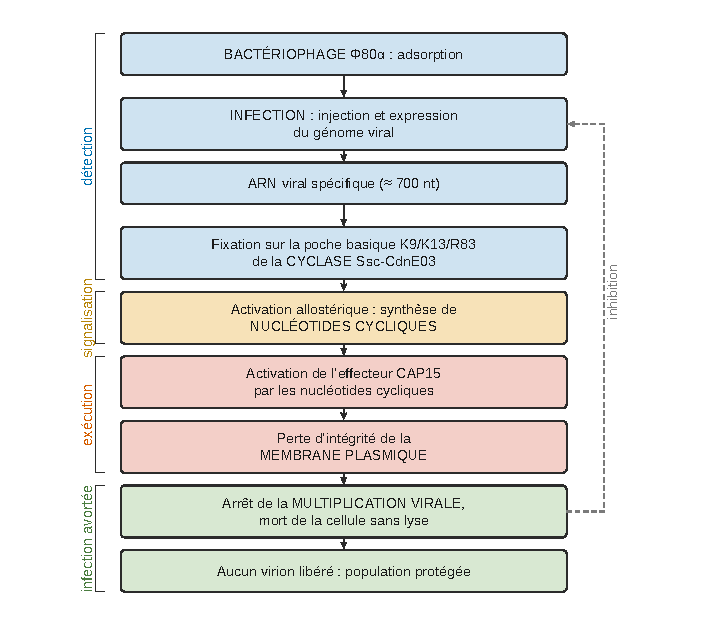
\includegraphics{figures/q28-logigramme-cbass.pdf}
\caption*{Figure 4 --- Logigramme de la cascade CBASS : un ARN viral active la
cyclase, les nucléotides cycliques activent CAP15, la membrane plasmique
est perméabilisée et la multiplication virale s'arrête}
\end{figure}

\equationajustee{\boxed{\textbf{\text{bactériophage}} \rightarrow \textbf{infection} \rightarrow \text{ARN viral} \rightarrow \textbf{cyclase} \rightarrow \textbf{\text{nucléotides} cycliques} \rightarrow \textbf{CAP15} \rightarrow \textbf{membrane plasmique} \rightarrow \text{\text{arrêt} de la } \textbf{multiplication virale}}}

\hypertarget{q29.-lien-avec-la-mort-cellulaire-par-apoptose-chez-lhomme}{%
\subsection{Q29. Lien avec la mort cellulaire par apoptose chez l'Homme}\label{q29.-lien-avec-la-mort-cellulaire-par-apoptose-chez-lhomme}}

\textbf{1. Une même logique fonctionnelle.} L'apoptose est une \textbf{mort cellulaire programmée}, génétiquement encodée, déclenchée par la cellule elle-même lorsqu'elle détecte une anomalie irréparable --- lésion de l'ADN, stress du réticulum, et notamment \textbf{infection virale}. Comme le CBASS, c'est un \textbf{sacrifice individuel au bénéfice de l'ensemble} : une cellule infectée qui s'autodétruit avant la fin du cycle viral n'engendre pas de descendance virale et protège l'organisme entier, exactement comme la bactérie \emph{Ssc}-CBASS protège sa population. Dans les deux cas, le principe est celui de l'\textbf{infection avortée}.

\textbf{2. Une même architecture en trois modules.}

\begin{longtable}[]{@{}
  >{\raggedright\arraybackslash}p{(\columnwidth - 4\tabcolsep) * \real{0.1830}}
  >{\raggedright\arraybackslash}p{(\columnwidth - 4\tabcolsep) * \real{0.2744}}
  >{\raggedright\arraybackslash}p{(\columnwidth - 4\tabcolsep) * \real{0.5126}}@{}}
\toprule\noalign{}
\begin{minipage}[b]{\linewidth}\raggedright
Module
\end{minipage} & \begin{minipage}[b]{\linewidth}\raggedright
CBASS bactérien
\end{minipage} & \begin{minipage}[b]{\linewidth}\raggedright
Immunité innée et apoptose chez l'Homme
\end{minipage} \\
\midrule\noalign{}
\endhead
\bottomrule\noalign{}
\endlastfoot
Détection du non-soi & Cyclase Ssc-CdnE03 liant un \textbf{ARN viral} & \textbf{cGAS} liant l'ADN cytosolique ; RIG-I et MDA5 liant l'ARN viral ; récepteurs de type Toll \\
Second messager & \textbf{Oligonucléotides cycliques} & \textbf{2′3′-cGAMP} produit par cGAS, reconnu par \textbf{STING} \\
Exécution & \textbf{CAP15}, qui perméabilise la membrane plasmique & \textbf{BAX/BAK}, qui perméabilisent la membrane mitochondriale externe (puis cytochrome \emph{c} et caspases) ; \textbf{gasdermines}, qui perforent la membrane plasmique (pyroptose) \\
\end{longtable}

\textbf{3. Une parenté évolutive, et pas seulement une analogie.} Les cyclases bactériennes de ce type appartiennent à la famille des \textbf{CD-NTases}, dont la cGAS humaine est un membre : même repliement, même chimie, même type de produit. Des domaines apparentés à \textbf{STING} et des \textbf{gasdermines} bactériennes ont été décrits dans des opérons de défense procaryotes. L'interprétation communément admise est que le système cGAS--STING des animaux \textbf{descend} de systèmes de défense antiphagiques procaryotes, ultérieurement complexifiés --- ce que signale d'ailleurs le titre de l'article source cité dans la bibliographie du sujet, \emph{Bacterial cGAS senses a viral RNA to initiate immunity}.

\textbf{4. Les limites du parallèle.}

\begin{itemize}
\tightlist
\item
  L'apoptose \emph{stricto sensu} est une mort \textbf{non inflammatoire} qui \textbf{préserve l'intégrité de la membrane plasmique} jusqu'aux stades tardifs : la cellule apoptotique se fragmente en corps apoptotiques phagocytés et reste d'abord non marquée par l'iodure de propidium. Or, ici, l'entrée précoce du marqueur signale justement une perte d'étanchéité : le phénotype observé s'apparente davantage à la \textbf{pyroptose} ou à la \textbf{nécroptose} qu'à l'apoptose canonique.
\item
  L'apoptose repose sur une cascade de \textbf{caspases}, dont aucun équivalent n'apparaît dans le CBASS étudié.
\item
  Une bactérie est unicellulaire : le bénéficiaire du sacrifice n'est pas un organisme mais un \textbf{clone}, ce qui déplace la question évolutive vers la sélection de parentèle.
\item
  Enfin, l'apoptose intervient aussi dans le \textbf{développement} (morphogenèse, sélection des lymphocytes), fonction sans équivalent bactérien.
\end{itemize}

On évitera donc d'écrire que les bactéries « font de l'apoptose » : elles réalisent une mort cellulaire programmée, ce qui n'est pas la même chose.

\equationajustee{\boxed{\text{\text{Même} logique de suicide altruiste face \text{à} l'infection, \text{même} architecture senseur} \rightarrow \text{\text{nucléotide} cyclique} \rightarrow \text{effecteur \text{perméabilisant} ; le couple cGAS–STING humain en est l'\text{héritier} \text{évolutif}.}}}

\end{document}
